\chapter[Appendix: Train Track Case Analysis: Track 0]{Train Track Case Analysis: Track 0}
\label{app:case_analysis_track0}


Here is Track 0:
\bigskip
\begin{figure}[H]
    \centering
    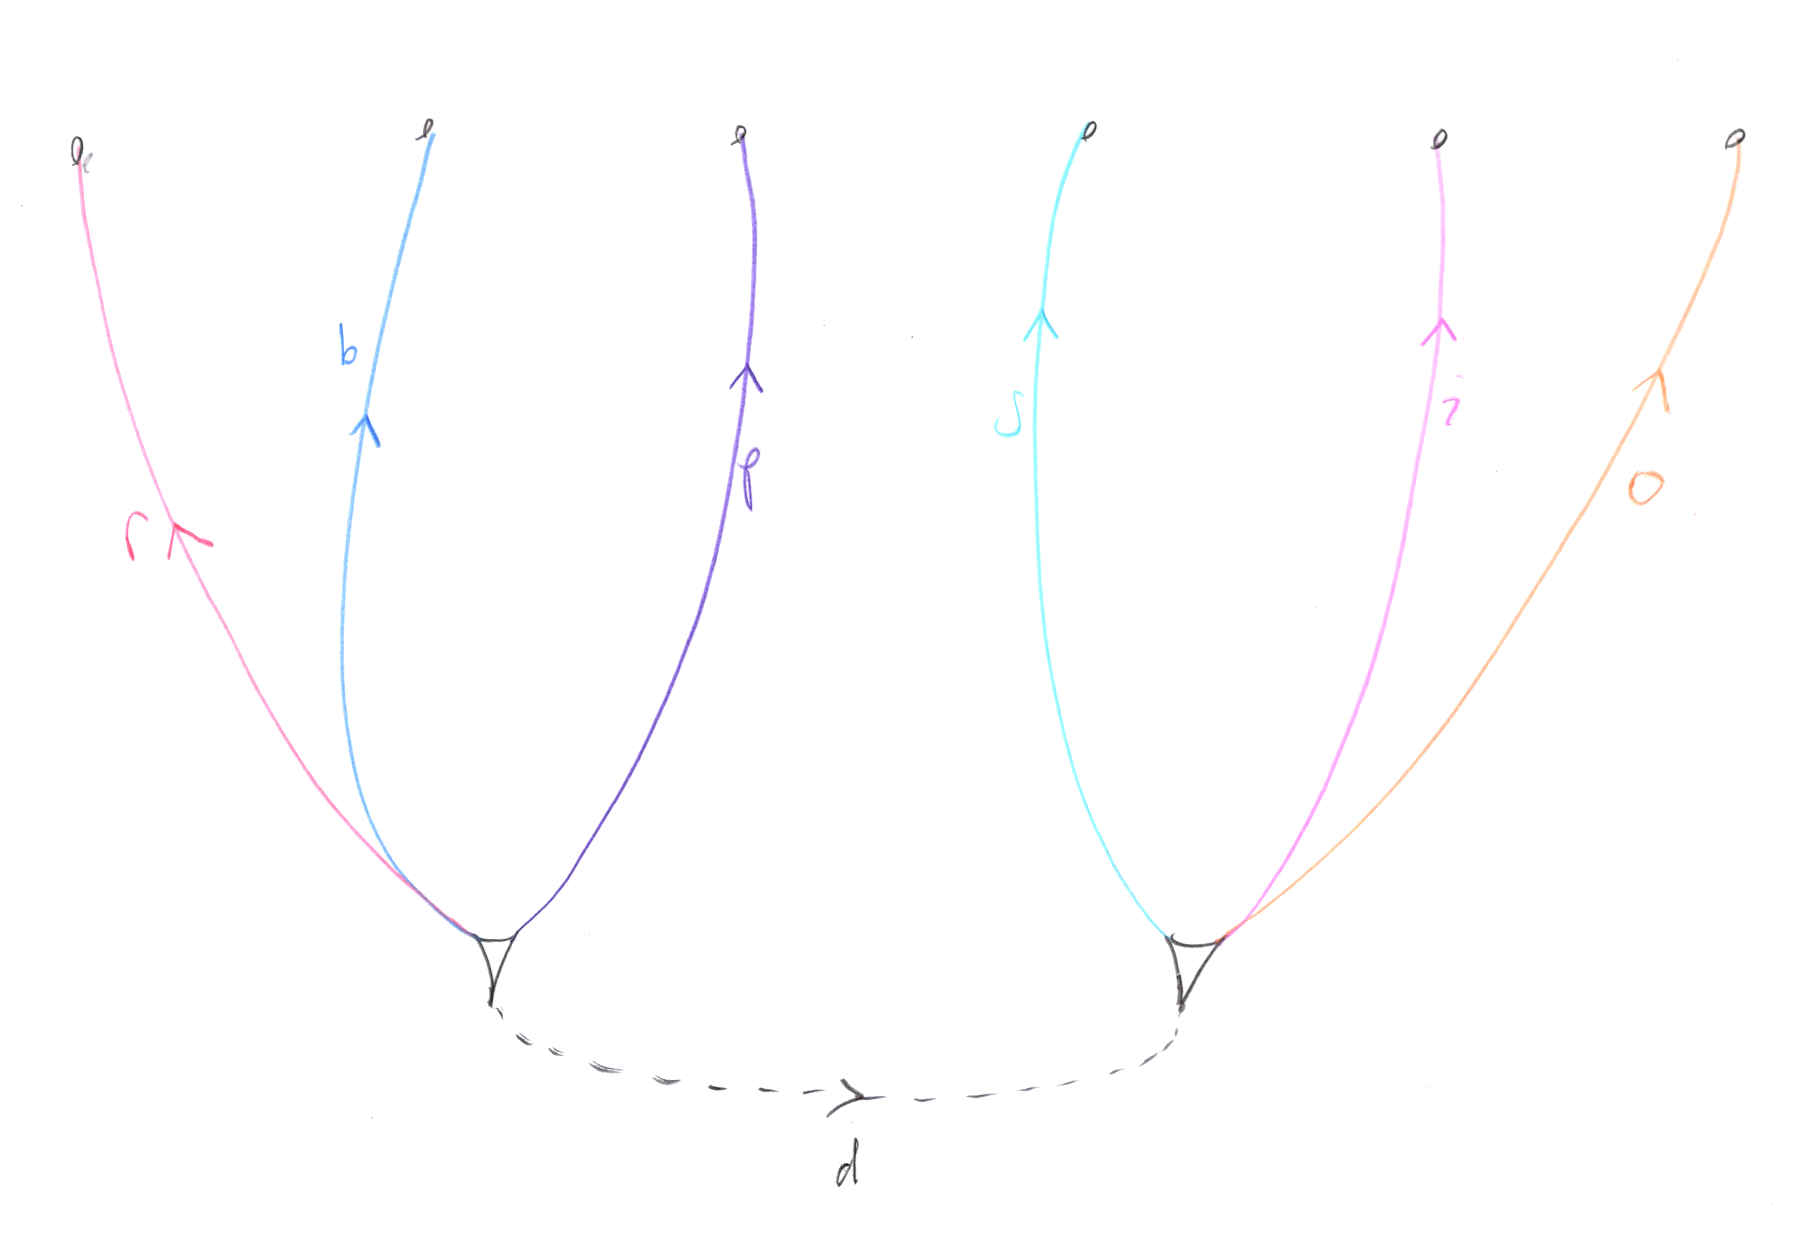
\includegraphics[width=\textwidth]{./traintrackdiagrams/Track0/track0.png}
    \sidecaption[][-0.5cm]{Track 0
    \label{fig:track0}}
\end{figure}

\section{Case A: Triangles fixed} \label{CaseA:Track0}
Triangles are fixed, and $f_\beta(d)$ and $f_\beta (\overline{d})$ both pass over $d$ after an even number of letters, we will call this \textit{Assumption A}. We know $f_\beta$ does not start at $d$, and $f_\beta(\overline{d})$ does not start at $\overline{d}$, otherwise $p$ and $s$ would pass over themselves. 

Thus $f_\beta(d)$ must start at $r,b,$ or $p$; and $f_\beta(\overline{d})$ must start at $s,i,$ or $o$.

Furthermore, notice that Track 0 is isomorphic to its own mirror, so there is the following symmetry: a train track map, carried by a braid $\beta$ yields from among the case analysis under the assumption that $\fbd$ begins with $r$ and $\fbdb$ begins with $i$ if and only if one carried by $\bar{\beta}$ yields from among the case analysis under the assumption that $\fbd$ begins with $b$ and $\fbdb$ begins with $o$. 


Indeed, it is clear that $\beta$ also carries a train track map on the mirror of Track 0, 

\subsection{AVX}\label{AVX}
Suppose $\fbd$ starts at $r$ and $\fbdb$ starts at $s$.

This is AVX1.

Here notice that $\fbd$ must eventually traverse $p^- d...$ in order to meet Assumption A, and in fact it must do so without any prior initial twists with $b$. Otherwise it would bring $\fbb$ along and cause it to trace. So we must have 
\[
\fbd = r^- p^- d...
\]
as depicted in AVX2.

Notice also that $\fbdb$ must begin with $s^-$ to meet Assumption A.

Here $\fbr$ can begin with $p^-$ or $p^\circ$
\subsubsection{Phil} \label{Phil}
Suppose $\fbr$ begins with $p^-$. Then we have Phil1.

Here $\fbdb$ can continue with $i^-$ or $o^-$.
\subsubsubsection{Linen} \label{Linen}
Suppose $\fbdb$ continues with $i^-$. Then we must have
\[
\fbdb = s^- o^- \dbar...
\]

This is Linen1.

Here the dotted lines can either join, or $\fbd$ must continue into 1., 2., or 3. labeled in the diagram. Note here that $\fbd$ cannot continue between $\fbo$ and $\fbi$ (the orange and pink edges) since it will be absorbed.

\subsubsubsubsection{Bibble}\label{Bibble}
Suppose dotted lines join. Then $\fbr$ is forced to continue with $di^*...$, and it cannot go to $o^*$ after crossing $d$, as that would force wither itself to trace if it goes $o^-$, or forcing $f_\beta(p)$ to trace. Then $\fbr$ continues with $s^+ \dbar p^+b^*$. So we have 
\[
f_\beta(r) = p^-di^+s^+\overline{d}p^+b^*...
\]

This forces $f_\beta(p)$ to end at $o^\circ$:
\[
f_\beta(p) = do^\circ
\]
or else it will trace. 

On the other hand, $f_\beta(i)$ has to be
\[
f_\beta(i) = \overline{d}p^+...
\]
and continue with $r^*$ or $b^*$.

This is Bibble1.

\subsubsubsubsubsection{Bawcock}
Suppose $f_\beta(i)$ continue with $r^*$. Then the following is forced:

Bawcock1.

Here $f_\beta(i)$ is forced to go
\[
f_\beta(i) = \overline{d}p^+r^+do^+\overline{d}...
\]
Thus $f_\beta(b)$ cannot simply be $f_\beta(p^\circ)$ because then $f_\beta(i)$ will be absorbed; nor can it start with $f_\beta(b) = p^+$ because then itself will be absorbed. Hence we have $f_\beta(b) = p^-...$ and continues with $f_\beta(b) = p^-d...$. At this point it can continue with either $o^-$ or $i^+$ but the former will trace, so it continues with $o^-$:
\[
f_\beta(b) = p^-do^-\overline{d}r^-p^-...
\]
but now it is absorbed. 


and $f_\beta(b)$ is absorbed. This is a contradiction.

\subsubsubsubsubsection{Chaffer}
Back to the end of Bibble \ref{Bibble}. Suppose $f_\beta(i)$ continues with $b^*$. 

This is Chaffer1.

In this case it has to be in fact $b^\circ$, otherwise it will trace. So we have
\[
\fbi = \dbar p^+b^\circ.
\]

This forces the situation depicted in Chaffer2.


Now consider $\fbs$, which starts with $i^*$. It cannot start with $i^+$, or it will immediately trace. We claim that it can also not start with $i^-$. Suppose it did. Then the following is forced:
\[
\fbs = i^-\dbar p^+r^+ d o^+ p^*...
\]
At this point $\fbb$ is forced to begin with $p^-$, or $\fbs$ will be absorbed. So we have
\[
\fbb = p^-di^*
\]
And now $\fbo$, which we know at this point is
\[
\fbo = \overline{d}p^+b^+p^+di^*
\]
must continue with $i^-$, otherwise $\fbb$ will trace. Thus we have
\[
\fbo = \overline{d}p^+b^+p^+di^-...
\]
but now $\fbo$ will trace as the following is forced:
\[
\fbo = \overline{d}p^+b^+p^+di^-\dbar p^+r^+do^*
\]
This is a contradiction. Thus $\fbs$ must start (and end) with $i^\circ$:
\[
\fbs = i^\circ.
\]

This is Chaffer3.

Here $\fbo$ must continue with $s^-$ and to the right of $\fbr$. Otherwise, $\fbr$ would continue with $s^+$ and to the left of $\fbo$, in which case, it would be absorbed:
\[
\fbr = ...s^+ i^- \dbar p^+ b^- p^- d \Abso{\fbo}{\fbi}
\]

So we must have
\[
\fbo =...s^- i^- \dbar p^+ b^- p^- d s^- i^- \dbar p^*...
\]
as shown in Chaffer4.

Here the incoming $\fbo$ forces $\fbb$ to begin with $p^-$ and to the right of $\fbo$. But now it will trace:
\[
\fbb = p^- d i^+ s^+ \dbar p^+ b^\times
\]

This is a contradiction.

\subsubsubsubsection{Fangle}
Back to the end of Linen \ref{Linen}
. Suppose dotted lines do not join, and suppose $\fbd$ goes into 1.

This is Fangle1.

Here neither of the dotted lines can traverse above $\fbp$, or they would enter into Situation $\beta$. So they circle the perimeter, and will be in Situation $\alpha$.

This is a contradiction.


\subsubsubsubsection{Hallan}
Back to the end of Linen \ref{Linen}. Suppose dotted lines do not join, and suppose $\fbd$ goes into 2. But in this case, $\fbd$ is immediately in Situation $\beta$. 

This is a contradiction.

\subsubsubsubsection{Jargle}
Back to the end of Linen \ref{Linen}. Suppose dotted lines do not join, and suppose $\fbd$ goes into 3. 

Then the situation is shown in Jargle1.

Where $\fbd$ must continue with $p^+$ after crossing $d$ and not $o$ to not violate Rule F1.

Here $\fbd$ continues with $\dbar p^+$, and the next letter cannot be $b^*$ or it would violate Rule F1. So the next letter must be $r^+$, and then:
\[
\fbdb = s^- i^- \dbar p^+ \hat{r}^+ d o^+...
\]
where it just violated Rule F1.

This is a contradiction.

\subsubsubsection{Kedge}
Back to \ref{Phil} Phil. Suppose $\fbdb$ continues with $o^-$. 

This is Kedge1.

Here if $\fbdb$ went above $\fbp$ in the middle, then $\fbp$ will trace:
\[
\fbp = d o^+ s^+ \dbar p^\times
\]

So $\fbdb$ msut go below $\fbp$ to give the situation in Kedge2.

Here both dotted lines cannot go below $\fbo$ and $\fbi$ or they would enter Situation $\beta$. So they go above, and will be in Situation $\alpha$.

This is a contradiction.


\subsubsection{Test} \label{Test}
Back to the end of AVX \ref{AVX}. Suppose 
\[
\fbr = p^\circf
\]

This is Test1.

Similar to the previous situations, here $\fbdb$ can continue with $i^-$ or $o^-$.

\subsubsubsection{Pugil} \label{Pugil}
Suppose $\fbdb$ continues with $i^-$.

This is Pugil1.

Here the dotted lines can join in the middle or $\fbd$ goes into 1. or 2. Note that it is impossible for it to go in between $\fbi$ and $\fbdb$ as that would cause it to enter Situation $\beta$.

\subsubsubsubsection{Limmer} \label{Limmer}
Suppose the dotted lines join in the middle. 

This is Limmer1.

Consider $\fbp$. After $\fbp = d...$, we must have
\[
\fbp = d o^*
\]
as $\fbp = d i$ will cause it to trace. In fact, it must be
\[
\fbp = d o^\circ
\]
since both $d o^-$ and $d o^+$ will cause $\fbp$ to trace.

Now consider $\fbo$. We must have
\[
\fbo \overline{d} p^+ b^*...
\]
Here it cannot go $\fbo \overline{d} p r^*...$ as it will then trace.

Now consider $\fbi$. We have either
\[
\fbi = \dbar p^+ r^*...
\]
or 
\[
\fbi = \dbar p^+ b^*...
\]

\subsubsubsubsubsection{Costard}
Suppose 
\[
\fbi = \dbar p^+ r^*...
\]

Then $\fbi$ continues:
\[
\fbi = \dbar p^+ r^+ d o^+ \dbar p^+ r^*
\]

This is Coastard1.

Consider $\fbb$. We have
\[
\fbb = p^+ r^*...
\]
and here if $\fbb = p^+ r^\circ$ or  $\fbb = p^+ r^+$ will cause $\fbi$ to be absorbed between $\fbr$ and $\fbb$. Hence we must have $\fbb = p^+ r^-...$, and continue with

\[
\fbb = p^+ r^-p^- d o^- \dbar p^-...
\]
but now $\fbb$ is absorbed between $\fbo$ and $\fbi$.

This is a contradiction


\subsubsubsubsubsection{Daddock} \label{Daddock}
Back to the end of Limmer \ref{Limmer}
Suppose 
\[
\fbi = \dbar p^+ b^*...
\]

Then in fact $\fbi$ must end there:
\[
\fbi = \dbar p^+ b^\circ.
\]

This is because both $\fbi = \dbar p^+ b^+$ and $\fbi = \dbar p^+ b^-$ will cause it to trace, or absorbed:
\[
\fbi = \dbar p^+ b^+ p^- d i^\times
\]

\[
\fbi = \dbar p^+ b^- p^- d  s^- i^\times
\]
or 
\[
\fbi = \dbar p^+ b^- p^- \times
\]

So we have the situation depicted in Daddock1.

Consider $\fbo$. We have 
\[
\fbo = \dbar p^+ b^+ p^- d i^*...
\]

Consider $\fbs$. We cannot have $\fbs = i^+...$ because it will immediately trace.
Thus we must have either
\[
\fbs = i^-
\]
or
\[
\fbs = i^\circ
\]
\subsubsubsubsubsubsection{Cordwain}
Suppose 
\[
\fbs = i^-...
\]

Then right after $i^-$, $\fbs$ must go to the right of $\fbo$ or else it will eventually be absorbed between $\fbo$ and $\fbi$. Continuing, we have
\[
\fbs = i^- \dbar p^+...
\]
Here it cannot go up $b$: $\fbs = i^- \dbar p^+ b^-...$, as this would make it eventually trace:
\[
\fbs = i^- \dbar p^+ b^-p^- d s^\times
\]
Thus we must have
\[
\fbs = i^- \dbar p^+r^+ d o^+ \dbar p^+r^*...
\]

This is Cordwain1.

Now consider $\fbb$. We have
\[
\fbb = p^+r^*
\]
and here if we have $\fbb = p^+r^\circ$ or $\fbb = p^+r^+$, then $\fbs$ will be forced to continue with $\fbs = i^- \dbar p^+r^+ d o^+ \dbar p^+r^+...$, which would immediately lead to $\fbs$ being absorbed between $\fbr$ and $\fbb$. Thus we must have $\fbb = p^+r^-...$, and continue to the right side of $\fbs$ as it comes down.


Now the following is forced, and it is eventually absorbed:
\[
\fbb = p^+r^-p^- d o^- \dbar r^-p^- d i^*
\]

This is Cordwain2.

Consider $\fbo$. Here $\fbo$ cannot continue with $i^\circ$ or $i^+$ as this will force $\fbb$ to continue with $i^+$ as well, and it will be absorbed:

\[
\fbb = p^+r^-p^- d o^- \dbar r^-p^- d i^+\dbar p^+ b^- p^- d \Abso{\fbo}{\fbi}
\]
Similarly, $\fbo$ cannot continue with $i^+$ or it will also be absorbed between itself and $\fbi$:
\[
\fbo = \dbar p^+ b^+ p^- d i^+\dbar p^+b^-p^- d \Abso{\fbo}{\fbi}
\]

This is a contradiction.


\subsubsubsubsubsubsection{Loblolly}\label{Loblolly}
Back to end of Daddock \ref{Daddock}. Suppose 
\[
\fbs = i^\circ
\]
Then $\fbo$ continues with $i^+$:
\[
\fbo = \dbar p^+ b^+ p^- d i^+ s^*
\]

The situation now is shown in Loblolly1.


Here $\fbo$ cannot continue with $s^+$ or it will be absorbed:
\[
\fbo = \dbar p^+ b^+ p^- d i^+ s^+ i^- \dbar p^+b^- p^- d \Abso{\fbo}{\fbi}
\]

Also, $\fbb$ cannot continue with $r^+$ or it will be absorbed:
\[
\fbb = p^+ r^+ p^- \Abso{\fbo}{\fbb}
\]

Thus we must have 
\[
\fbo = \dbar p^+ b^+ p^- d i^+ s^{\substack{\circ \\[ -3pt] -}}...
\]
and
\[
\fbb = p^+r^{\substack{\circ \\[ -3pt] -}}...
\]

However, suppose $\fbo$ goes $s^-$, then we have
\[
\fbo = \fbo = \dbar p^+ b^+ p^- d i^+ s^-i^-\dbar p^+ b^- p^+ d s^- i^-  \dbar p^+ r^*...
\]
and now this forces $\fbb$ to go $r^-$, as ending with $r^\circ$ here will force $\fbo$ to be absorbed. But now we have
\[
\fbb = p^+r^-p^+ d i^+ s^+ i^- \dbar p^+ b^- p^- d \Abso{\fbo}{\fbi}
\]

% See Figure \ref{WingA}

Thus $\fbo$ cannot go $s^-$, and so we must have
\[
\fbo = \fbo = \dbar p^+ b^+ p^- d i^+ s^\circ
\]

This is Loblolly2.

But now this also forces $\fbb$ to end with $r^\circ$; as going $r^-$ now will be absorbed:
\[
\fbb = po^+r^- p^-  d i^+s^+ i^- \dbar p^+ b^- p^- d \Abso{\fbo}{\fbi}
\]

The conclusion is that we must have
\[
\fbo = \fbo = \dbar p^+ b^+ p^- d i^+ s^\circ
\]
and
\[
\fbb = p^+r^\circ
\]

This gives Candidate 1. Shown in Loblolly3.

\subsubsubsubsection{Smouch}
Back to the end of Pugil \ref{Pugil}. Suppose $\fbs$ goes into 1.

This is Smouch1.

Here both $\fbd$ and $\fbdb$ in the middle cannot go above $\fbp$ or it would enter Situation $\beta$. So they both continue with $r^-$ and will be in Situation $\alpha$.

This is a contradiction.

\subsubsubsubsection{Thwite}
Back to the end of Pugil \ref{Pugil}. Suppose $\fbs$ goes into 2, after which it must go up $i$ and not $o$, or it will have to cross $\dbar$ again immediately, which is not allowed. Then we have
\[
\fbd = r^- p^- d i^+ s^+ \dbar p^+...
\]
and
\[
\fbdb = s^- i^- \dbar p^+...
\]

as shown in Thwite1.

At this point neither of these can go up $b$, as that will force them to violate Rule F1. Hence both have to continue clockwise, with $...r^+ d o...$. 

But then they will cross $d$ and then traverse $o^+ \dbar$, thereby violating Rule F1.

This is a contradiction.

\subsubsubsection{Quarl} \label{Quarl}
Back to end of Test \ref{Test}. Suppose $\fbdb$ continue with $o^-$, so we have the situation shown in Quarl1.

Here the dotted lines can join, or $\fbd$ goes into 1 or 2. Again it cannot go in between $\fbi$ and $\fbdb$ or it would be in Situation $\beta$.

\subsubsubsubsection{Wamble}
Suppose the dotted lines join, or $\fbd$ goes into 2. In both cases we have
\[
\fbp = d o^+ s^+ \dbar p^\times
\]
This is a contradiction.


\subsubsubsubsection{Yaffle}
Back to end of Quarl (\ref{Quarl}). Suppose $\fbd$ goes into 1. In this case $\fbdb$ has to go under $\fbp$ otherwise it would enter Situation $\beta$.

Now $\fbd$ continues:
\[
\fbd = r^- p^- d s^- o^- \dbar...
\]

Giving us Yaffle1.

But now the dotted lines have no means of joining, and they continue clockwise in the outer perimeter indefinitely, they are in Situation $\alpha$.

This is a contradiction.




\subsection{ACK} \label{ACK}
Back to the end of Case A (\ref{CaseA:Track0}). Suppose $\fbd$ begins with $r$, and $\fbdb$ begins with $i$. We remind the reader that Assumption A must still be held, that is, both $\fbd$ and $\fbdb$ must go over an even number of letters before crossing.

The situation is shown in ACK1.

Notice that both $\fbd$ and $\fbdb$ traverse only twice before crossing, since any additional twists would cause tracing.

Here the dotted lines can join, or $\fbd$ can go into 1 or 2.

\subsubsection{Dram} \label{Dram}
Suppose the dotted lines join. 

This is Dram1.

Here $\fbs$ cannot go below $\fbp$, or it would trace:
\[
\fbs = \dbar r^- p^- d s^\times
\]

So we have
\[
\fbs = \dbar p^*
\]

Separately, consider $\fbp$. It starts with $d$, and cannot continue with $i$, or it will trace:
\[
\fbp = d i^+ s^+ \dbar p^\times
\]
Thus we must have
\[
\fbp = d o^*
\]
Here, if it is $o^+$, then $\fbp$ traces:
\[
\fbp = d o^+ \dbar p^\times
\]
Similarly, if it is $o^-$, $\fbp$ also traces:
\[
\fbp = d o^- \dbar r^- p^\times
\]
Therefore we must have
\[
\fbp = d o^\circ
\]

This is Dram2.

Consider $\fbr$ and $\fbb$. They both start with $p$:
\[
\fbr = p^*...
\]
\[
\fbb = p^*...
\]

Consider $\fbo$. We have
\[
\fbo = s^+ \dbar  p^*
\]
and here is we have $p^\circ$ or $p^-$, $\fbs$ will be forced to go $p^-$, and it will trace:
\[
\fbs = \dbar p^- d s^\times
\]
Thus we must have
\[
\fbo = s^+ \dbar  p^+...
\]
and $\fbo$ then goes into 1 or 2. 

\subsubsubsection{Sloom}\label{Sloom}
Suppose $\fbo$ continues into 1. Then it continues with the following:
\[
\fbo = s^+ \dbar p^+ d i^+ s^+ \dbar p^+...
\]
Here the next letter cannot be $r$, or we will trace:
\[
\fbo = s^+ \dbar p^+ d i^+ s^+ \dbar p^+ r^+ d o^\times
\]
Thus we must have
\[
\fbo = s^+ \dbar p^+ d i^+ s^+ \dbar p^+ b^*...
\]

Now consider $\fbr$ and $\fbb$. They both start out similarly:
\[
\fbr = p^- d s^- i^*...
\]
\[
\fbb = p^- d s^- i^*...
\]

This is Sloom1.

Consider $\fbs$. It must end at $p^\circ$. Indeed, if after $\dbar$ it goes  $p^-$ it will trace almost immediately:
\[
\fbs = \dbar p^- d s^\times
\]
Similarly, if it goes $p^+$:
\[
\fbs = \dbar p^+ d i^+ s^\times
\]
Hence we have
\[
\fbs = \dbar p^\circ
\]

This is Sloom2.

Consider $\fbi$. It must end immediately at $s^\circ$. Indeed, $\fbi = s^-...$ will immediately cause it to be absorbed between itself and $\fbo$; if it starts with $s^+$, then
\[
\fbi = s^+ \dbar p^+ d i\times
\]
Therefore we must have
\[
\fbi = s^\circ
\]

The situation now is depicted in Sloom3.

Here $\fbb$ can either end with $i^\circ$ or continue with $i^+$. It cannot continue with $i^-$ as that would cause it to escape to the outer perimeter and eventually trace, due to the position of $\fbo$. 

Suppose it ended at $i^\circ$. Then $\fbr$ continues:
\[
\fbr = ...i^- s^+ \dbar p^+ d i^+ s^+ \dbar p^+ b^*...
\]
as shown in Sloom4.

Here if $\fbo$ continue with $b^\circ$ or $b^+$, forcing $\fbr$ to continue with $b^+$, then $\fbr$ would eventually be absorbed:
\[
\fbr = ...b^+ p^- d s^- i^- \dbar p^- d s^- \Abso{\fbi}{\fbo}
\]

So $\fbo$ must continue with $b^-$ and to the right of $\fbr$. But now it will be absorbed:
\[
\fbo = ...b^- p^- d s^- i^- \dbar p^-d s^- i^+ s^+ \dbar p^+ \Abso{\fbr}{\fbb}
\]

So in fact $\fbb$ cannot end at $i^\circ$. So suppose it continued with $i^+$. Then we have
\[
\fbb = p^- d s^- \hat{i}^+ s^+ \dbar p^+ r^*...
\]

as shown in Sloom5.

Here $\fbr$ must end immediately, as continuing otherwise would cause it to follow $\fbb$ and trace eventually.

This in turn forces $\fbb$ to end as well. As otherwise it would either be absorbed between $\fbb$ and $\fbr$, or escape to the outer perimeter.

Lastly, these two ending this forces $\fbo$ to end as well. Otherwise, it would traverse back and eventually be absorbed.

This gives us Candidate 2.



% Here let us consider $\fbr$ again. There are only three letters available left for $\fbr$ to end at: $i$, $b$, or $r$; so it must end at either $i$ or $b$ to not trace. Similarly, $\fbb$ must end at $i$ or $r$. 

% Furthermore, notice that if $\fbr$ does not end at $i$, then it has to go $i^-$ because going $i^+$ will bring it to $r$ and trace. Similarly, if $\fbb$ does not end at $i$, it has to go $i^+$ or either trace: 
% \[
% \fbb = p^- d s^- i^- s^+ \dbar p^+ d i^+ s^+ \dbar p^+ b^\times
% \]
% or get absorbed:
% \[
% \fbb = p^- d s^- i^- s^+ \dbar p^+ d o^- \dbar r^- p^- d s^- i^- \dbar p^- d s^- \Abso{\fbi}{\fbo}
% \]

% Now if $\fbr$ does not end at $i$, it continues with $i^-$, and note that it has to come down to the right of $\fbb$:
% \[
% \fbr = \fbr = p^- d s^- i^- s^+ \dbar p^+ d i^+ s^+ \dbar p^+ b^*...
% \]
% This is shown in Figure.

% Let us consider $\fbb$ again. If it does not end at $i$ at this point, as mentioned before, it has to go $i^+$. But now the position of $\fbr$ will causes it to be absorbed:
% \[
% \fbb = p^- d s^- i^+ s^+ \dbar p^+ \Abso{\fbr}{\fbb}
% \]
% Therefore, in this case, $\fbb$ must end at $i$:
% \[
% \fbb = p^- d s^- i^\circ
% \]

% Now consider $\fbr$ again. Suppose now it continues with $b^+$. If this were done by going to the right of $\fbo$, will trace:
% \[
% \fbr = \fbr = p^- d s^- i^- s^+ \dbar p^+ d i^+ s^+ \dbar p^+ b^+  p^- d s^- i^- \dbar p^- d s^- i^+ s^+ \dbar p^+ r^\times 
% \]
% If this were done to the left of $\fbo$, then it's absorbed:
% \fbr = \fbr = p^- d s^- i^- s^+ \dbar p^+ d i^+ s^+ \dbar p^+ b^+ p^- d s^- i^- \dbar p^- d s^- \Abso{\fbi}{\fbo}
% \]

% On the other hand, if $\fbr$ were to continue with $b^-$, then it will come back to $i$, forced to go $i^+$ by the position of $\fbb$, and eventually be absorbed:
% \[
% \fbr = p^- d s^- i^- s^+ \dbar p^+ d i^+ s^+ \dbar p^+ b^- p^- d s^- i^- \dbar p^-  d s^- i^+ s^+ \dbar p^+ \Abso{\fbr}{\fbb}
% \]

% Therefore, we can conclude that $\fbr$ must end at $b$:
% \[
% \fbr = p^- d s^- i^- s^+ \dbar p^+ d i^+ s^+ \dbar p^+ b^\circ
% \]

% Now this immediately forces $\fbo$ to go $b^-$, which will lead to it being absorbed:
% \[
% \fbo = s^+ \dbar p^+ d i^+ s^+ \dbar p^+ b^- p^- d s^- i^- \dbar p^-  d s^- i^+ s^+ \dbar p^+ \Abso{\fbr}{\fbb}
% \]



% This can then be repeated any number of times before $\fbr$ eventually ends at either $i$ or $b$. So we have
% \[
% \fbr = p^- d s^- i^- ( s^+ \dbar p^+ d i^+ s^+ \dbar p^+ b^- p^- d s^-i^- \dbar p^- d s^-)^n i^\circ
% \]
% or
% \[
% \fbr = p^- d s^- i^-  s^+ \dbar p^+ d i^+ s^+ \dbar p^+ (b^- p^- d s^-i^- \dbar p^- d s^- i^- s^+ \dbar p^+ d i^+ s^+ \dbar p^+)b^\circ
% \]

% Therefore, in the situation depicted in Figure Mace1, $\fbr$ must end at $i$:
% \[
% \fbr = p^- d s^-i^\circ
% \]

% This then forces $\fbb$ to go $i^+$:
% \[
% \fbb = p^- d s^- i^+ s^+ \dbar p^+ r^*...
% \]
% This is depicted in Mace3.

% Now we claim that $\fbb$ has to end at $r$ here. Suppose in the contrary that it goes $r^+$. Then we have
% \[
% \fbb = p^- d s^- i^+ s^+ \dbar p^+ r^+ p^- d s^-i^- s^+ \dbar p^+ \Abso{\fbr}{\fbb}
% \]
% And if it were to go $r^-$:
% \[
% \fbb = p^- d s^- i^+ s^+ \dbar p^+ r^- p^- d s^-i^- s^+  \dbar p^+ d...
% \]
% here the next letter can be either $i^+$ or $o^-$, but the former will cause it to trace:
% \[
% \fbb = p^- d s^- i^+ s^+ \dbar p^+ r^- p^- d s^-i^- s^+  \dbar p^+ d i^+ s^+ \dbar p^+ b^\times
% \]
% so it must be $o^-$:
% \[
% \fbb = p^- d s^- i^+ s^+ \dbar p^+ r^- p^- d s^-i^- s^+  \dbar p^+ d o^- \dbar r^- p^- d s^- i^- \dbar p^- d d^- \Abso{\fbi}{\fbo}
% \]
% Thus in the situation depicted in Mace3, $\fbb$ must end at $r^\circ$.

% Now we only have $\fbo$ remaining. This is Mace4. We claim it has to end at $b^\circ$ in the situation depected in Mace4. If it were to go $b^-$, then
% \[
% \fbo = s^+ \dbar p^+ d i^+ s^+ \dbar p^+ b^- p^- d s^- i^- \dbar p^- d s^- i^+ s^+ \dbar p^+ r^+ p^- d s^-  i^- s^+ \dbar p^+ \Abso{\fbr}{\fbb}
% \]
% And if it were to go $b^+$, then
% \[
% \fbo = s^+ \dbar p^+ d i^+ s^+ \dbar p^+ b^+ p^- d s^- i^- \dbar p^- d s^- \Abso{\fbi}{\fbo}
% \]

% Hence in the situation depicted in Mace4, $\fbo$ ends at $b^\circ$.

% In conclusion, this gives our candidate train track map 0.2, shown in Mace5.


\subsubsubsection{Thrum}\label{Thrum}
Back to end of Dram (\ref{Dram}). Suppose $\fbo$ goes into 2. Then
\[
\fbo = s^+ \dbar p^+ r^*...
\]

This is Thrum1.

Here 
\[
\fbi = s^+
\]
or
\[
\fbi = s^\circ
\]
\subsubsubsubsection{Dwammy} \label{Dwammy}
Suppose $\fbi = s^+...$.

Then
\[
\fbi = s^+ \dbar p^+...
\]

Here if it were $p^\circ$ or $p^-$ then $\fbs$ will trace. Continuing:
\[
\fbi = s^+ \dbar p^+ r^*...
\]

This is Dwammy1.

Now consider $\fbo$. At this moment we have
\[
\fbo = s^+ \dbar p^+ r^*...
\]
Here if it were $r^\circ$ or $r^-$, $\fbi$ will be forced to go $r^-$ and eventually trace:
\[
\fbi = s^+ \dbar p^+ r^- p^- d s^- i^\times
\]
Hence we must have 
\[
\fbo = s^+ \dbar p^+ r^+...
\]
and continuing:
\[
\fbo = s^+ \dbar p^+ r^+ p*...
\]
This is Dwammy2.

Here if it were $p^\circ$ or $p^+$, then $\fbr$ will be forced to start with $p^+$, which would force it to immediately trace. Thus we must have
\[
\fbo = s^+ \dbar p^+ r^+ p^-...
\]
This situation is depicted in Dwammy3, and here $\fbo$ can go into 1 or 2 (it cannot go into the left of $\fbr$ as that would again force $\fbr$ to immediately trace).

\subsubsubsubsubsection{Macarize}
Suppose $\fbo$ goes into 1. Then it continues:
\[
\fbo = s^+ \dbar p^+ r^+ p^- d i^+ s^+ \dbar p^+ b^*...
\]
Here at the end it has to go to $b$ and not $r^+$ or it will trace. 

This is Macarize1.

Now consider $\fbs$. We have
\[
\fbs = \dbar p^+ r^*...
\]

Consider $\fbi$. Recall we have
\[
\fbi = s^+ \dbar p^+ r^*...
\]
Here if it were $r^\circ$ or $r^-$, then $\fbs$ will be forced to go $r^-$ and will trace:
\[
\fbs = \dbar p^+ r^- p^- d s^\times
\]
So it must be $r^+$. But now $\fbi$ traces:
\[
\fbi = s^+ \dbar p^+ r^+ p^- d i^\times
\]

This is a contradiction.

\subsubsubsubsubsection{Mooncalf}\label{Mooncalf}
Back to end of Dwammy (\ref{Dwammy}). Suppose $\fbo$ goes into 2. Then it continues:
\[
\fbo = s^+ \dbar p^+ r^+ p^- d s^*...
\]

The situation is depicted in Mooncalf1.

Now consider $\fbr$. It cannot start with $p^+$ or it will immediately trace. If it starts with $p^\circ$, then $\fbs$ will be forced to continue with $p^+$ as well and eventually trace:
\[
\fbs = \dbar p^+ r^- p^- d s^\times
\]
Thus, $\fbr$ starts with $p^-$:
\[
\fbr = p^- d s^*...
\]
and note that it has to go to the right of $\fbs$ to not cause $\fbs$ to trace again.

This is Mooncalf2.

Now consider $\fbb$. It cannot start with $p^+$, as the position of $\fbr$ (which is starting with $p^-$) prevents it from doing do without one of them getting absorbed immediately. It cannot start with $p^\circ$ either, as that would force $\fbs$ to be absorbed immediately between $\fbr$ and $\fbb$. Thus $\fbb$ also must start with $p^-$ as well, and also to the right of $\fbs$ to not cause it to be absorbed:
\[
\fbb = p^- d s^*...
\]

This is Mooncalf3.

Now consider $\fbs$. It must now end at $p^\circ$. Indeed, if it continues with either $p^+ d$ or $p^- d$ now it will immediately trace. Therefore we have
\[
\fbs = \dbar p^\circ
\]

This is Mooncalf4.

Now consider $\fbo = s^+ \dbar p^+ r^+ p^- d s^*...$. If it were $s^\circ$ or $s^+$, then $\fbr$ will trace:
\[
\fbr = p^- d s^+ \dbar p^+ r\times
\]
Thus it must be $s^-$ here. Then it continues:

\[
fbo = s^+ \dbar p^+ r^+ p^- d s^- \dbar p^+ d i^+ s^+ \dbar p^+...
\]
and here the next letter must be $b*$, and not $r^+$ since that will force it to go under $\fbp$ and as a result go up to $o$ with $\fbp$ and tracing. Thus we have
\[
\fbo = s^+ \dbar p^+ r^+ p^- d s^- \dbar p^+ d i^+ s^+ \dbar p^+ b^*...
\]

This is Mooncalf5.

Now consider $\fbi$. We have
\[
\fbi = s^+ \dbar p^+ r^*...
\]
Now if it were $r^-$ here, then it will be absorbed:
\[
bi = s^+ \dbar p^+ r^- p^- d s^- \Abso{\fbi}{\fbo}
\]
and if it were $r^+$, it traces:
\[
\fbi = s^+ \dbar p^+ r^+ p^- d s^- \dbar p^+ d i^\times
\]
Therefore $\fbi$ ends at $r^\circ$:
\[
\fbi = s^+ \dbar p^+ r^\circ
\]

This is Mooncalf6.

The situation now is depicted in Mind.

Now let us consider $\fbr$ and $\fbb$ again. We claim that $\fbr$ must end here at $s^\circ$. Suppose the contrary, then it cannot continue with $s^+$, as that would cause it to trace:
\[
\fbr = p^- d s^+ \dbar p^+ r^\times
\]
so in this case it has to continue with $s^-$. Suppose that were the case, then it has to go to the right of $\fbb$ as it comes down from $r^-$ otherwise it enters in between itself and $\fbb$ and thus will be absorbed eventually. Continuing, we have
\[
\fbr = p^- d s^- \dbar p^+ d...
\]
and here the next letter must be $i^+$ and not $o^-$ otherwise $\fbr$ will trace. Continuing:
\[
\fbr = p^- d s^- \dbar p^+ d i^+ s^+ \dbar p^+ b^*...
\]

Now consider $\fbb = p^- d s^*...$. If here it were $s^+$ then it will be absorbed between itself and $\fbr$. If it were $s^-$ then it will follow $\fbr$ and continue with
\[
\fbb = p^- d s^- \dbar p^+ d...
\]
but here the next letter must be $o^-$ or it will continue to follow $\fbr$ and eventually trace. But now we have
\[
\fbb = p^- d s^- \dbar p^+ d o^- \dbar r^- p^- d s^- o^- \dbar p^- d s^+ \dbar p^+ r^- p^- d s^- \Abso{\fbi}{\fbo}
\]

Therefore, we must have $\fbr$ ending at $s^\circ$:
\[
\fbr = p^- d s^\circ
\]

This is Mooncalf7.

Then this forces $\fbb$ to continue:
\[
\fbb = \fbb = p^- d s^+ \dbar p^+ r^- p^- d s^- o^*...
\]

Now at this point, we claim that $\fbb$ has to end here at $o^\circ$. Suppose not, and suppose it were $o^+$ instead. Then we have
\[
\fbb = \fbb = p^- d s^+ \dbar p^+ r^- p^- d s^- o^+ s^+ \dbar p^+ r^+ p^- d s^- \dbar p^+ \Abso{\fbr}{\fbb}
\]
and similarly if it were $o^-$:
\[
\fbb = p^- d s^+ \dbar p^+ r^- p^- d s^- o^- s^+ \dbar p^+ r^+ p^- d s^- \dbar p^+ d...
\]
and here it cannot continue with $i^+$ or it will follow $\fbo$ and trace. So instead it must continue with $o^-$, but then it will be absorbed:
\begin{align*}
    \fbb  =& p^- d s^+ \dbar p^+ r^- p^- d s^- o^- s^+ \dbar p^+ r^+ p^- d s^- \dbar p^+ d\\
    & o^- \dbar r^- p^- d s^- o^- \dbar p^- d s^+ \dbar p^+ r^- p^- d s^- \Abso{\fbi}{ \fbo} 
\end{align*}

Therefore, $\fbb$ has to end at $i^\circ$:
\[
\fbb = \fbb = p^- d s^+ \dbar p^+ r^- p^- d s^- o^\circ
\]

This is Mooncalf8.

Finally, let us consider $\fbo$. Recall we have
\[
\fbo = s^+ \dbar p^+ r^+ p^- d s^- \dbar p^+ d i^+ s^+ \dbar p^+ b^*...
\]
Now we claim that $\fbo$ has to end here at $b^\circ$. Indeed, if in the contrary it were $b^+$ here, then it will be absorbed:
\[
\fbo = ...b^+ p^- d s^- i^- \dbar p^- d s^+ \dbar p^+r^- p^- d s^- \Abso{\fbi}{\fbo}
\]
On the other hand, if it were $b^-$ instead, it will eventually follow $\fbb$ and thus trace:
\[
\fbo = ... b^- p^- d s^- i^- \dbar p^- d s^+ \dbar p^+ r^- p^- d s^- o^\times
\]

In conclusion, we have Candidate 3 shown in Mooncalf9.

\subsubsubsubsection{Faffel}\label{Faffel}
Back to the end of Thrum (\ref{Thrum}). Suppose $\fbi = s^\circ$. This is depicted in Faffel1.

Consider $\fbo$. We have

\[
\fbo = s^+ \dbar p^- r^*...
\]
and now this forces $\fbs$ to also continue with $p^-$. Indeed, if it continues with $p^\circ$ or $p^+$ instead, then both $\fbb$ and $\fbb$ will be absorbed between $\fbi$ and $\fbo$. So we have
\[
\fbs = \dbar p^+ r^*...
\]


Now the situation is depicted in Faffel2.

Now consider $\fbo$ again. Here it cannot continue with $r^\circ$ or $r^-$, as both will force $\fbs$ to continue with $r^-$, but that will force it to trace:
\[
\fbs = \fbs = \dbar p^+ r^- p^- d s^\times
\]

Thus, we must have
\[
\fbo = s^+ \dbar p^+ \hat{r}^+ p^- d i^+ s^+ \dbar p^+ b^*...
\]
and here it must go up $b^*$ and not $r^+$, or it will trace: $...r^+d o^\times$.

This is depicted in Faffel3.

Now consider $\fbs$. We claim that it has to end here at $r^\circ$. Suppose by the contrary, that it continues with $r^-$. Then we have
\[
\fbs = \dbar p^+ r^- p^- d s^\times
\]
Similarly, if it continues with $r^+$, then we have
\[
\fbs = \dbar p^+ r^+ p^- d s^\times
\]

So we must have
\[
\fbs = \dbar p^+ r\circ
\]

This is depicted in Faffel4.

Now consider $\fbo$ again. If here it continues with $b^+$, then it will be absorbed:
\[
\fbo = s^+ \dbar p^- r^+ p^- d i^+ s^+ \dbar p^+ b^+ p^- d s^- i^- \dbar p^+ r^- p^- d s^- \Abso{\fbi}{\fbo}
\]

On the other hand, if it continues with $b^-$, then we have
\[
\fbo =...\hat{b}^- p^- d s^- i^- \dbar p^*... 
\]
This is depicted in Faffel5. 

Now it cannot continue with $p^\circ$ or $p^-$, as that would force both $\fbb$ and $\fbr$ to continue with $p^-$, and both will then continue ``inside" $\fbo$, and eventually $\fbb$ will trace. On the other hand, if $\fbo$ were to continue with $p^+$ here, then it has to go to the left of $\fbb$ to not be absorbed, so then we have
\[
\fbo = s^+ \dbar p^- r^+ p^- d i^+ s^+ \dbar p^+ b^- p^- d s^- i^- \dbar \hat{p}^+ r^- p^- d s^- i^*... 
\]

This is depicted in Faffel6.

Now consider $\fbb$. If it starts with $p^\circ$ or $p^-$, then $\fbr$ will start with $p^-$ (and to the right of $\fbb$ to not be absorbed immediately):
\[
\fbr = p^- d...
\]
Now the next letter can be $o^-$ or $i^+$, but the former will make it trace:
\[
\fbr = p^- d o^- \dbar r^\times
\]
so the next letter must be $i^+$; but now it traces as well:
\[
\fbr = p^- d i^+ s^+ \dbar p^+ b^+ p^- d s^- i^- \dbar p^+  r^\times
\]

Therefore, in the situation depicted in Faffel6, $\fbb$ has to start with $p^+$, and this forces $\fbr$ to end at $p$ immediately in order to not trace or be absorbed:
\[
\fbr = p^\circ
\]
and $\fbb$ continues:
\[
\fbb = p^+ r^- p^- d s^- i^*...
\]
Now the situation is depicted in Faffel7.

Now if $\fbb$ continues with $i^\circ$ or $i^+$, then $\fbo$ continues with $i^+$, and it will be absorbed:
\[
\fbo = ...\hat{i}^+ s^+ \dbar p^+ r^+ p^- \Abso{\fbr}{\fbb}
\]

So in this situation depicted in Faffel7, $\fbb$ must continue with $i^-$, and to the right of $\fbo$, otherwise $\fbo$ will still be absorbed. But now $\fbb$ traces:
\[
\fbb = p^+ r^- p^- d s^- \hat{i}^- s^+ \dbar p^+ r^+ p^- d i^+ s^+ \dbar p^+ b^\times
\]

Therefore, we can conclude that in the situation depicted in Faffel4, $\fbo$ must end there at $b^\circ$. 

Now the situation depicted in Faffel8 is forced.

Consider $\fbr$. It cannot start with $p^+$ or it will immediately trace. So suppose it starts with $p^-$, and to the right of $\fbb$ to not be absorbed. Then we have
\[
\fbr = p^- d...
\]
Here the next letter can be either $o^-$ or $i^+$. The former will make $\fbr$ trace:
\[
\fbr = p^- d o^- \dbar r^\times
\]
so it must be the latter; but that also forces $\fbr$ to trace:
\[
\fbr = p^- d i^+ s^+ \dbar p^+ b^+ p^- d s^- i^- \dbar p^+ r\times
\]
Therefore, we must have, in the situation depicted in Faffel8, $\fbr$ starts and ends at $p^\circ$:
\[
\fbr = p^\circ
\]

Now this forces $\fbb$ to start with $p^+$ and continue:
\[
\fbb = p^+ r^- p^- d s^- i^*...
\]
This is depicted in Faffel9.

Now we claim that in fact $\fbb$ must end here at $i^\circ$. Suppose the contrary, and suppose $\fbb$ continues with $i^+$. Then we have
\[
\fbb = p^+ r^- p^- d s^- \hat{i}^+ s^+ \dbar p^+ r^+ p^- \Abso{\fbb}{\fbr}
\]

So suppose instead it continues with $i^-$. Then we have
\[
\fbb = p^+ r^- p^- d s^- \hat{i}^- s^+ \dbar p^+ r^+ p^- d...
\]
and here the next letter can be either $i^+$ or $o^+$, but the former will force it to trace:
\[
\fbb = p^+ r^- p^- d s^- \hat{i}^- s^+ \dbar p^+ r^+ p^- d i^+ s^+ \dbar p^+ b^\times
\]
so it must be the latter; but then it will be absorbed:
\[
\fbb = ...\hat{i}^- s^+ \dbar p^+ r^+ p^- d o^- \dbar r^- p^- d s^- i^- \dbar p^+ r^- p^- d s^- \Abso{\fbi}{\fbo}
\]

In conclusion, in the situation depicted in Faffel9, $\fbb$ must end there at $i^\circ$:
\[
\fbb = p^+ r^- p^- d s^- i^\circ
\]

This gives us our Candidate train track map 4. Depicted in Faffel10.

\subsubsection{Lugs}
Back to end of ACK (\ref{ACK}). Suppose $\fbd$ go into 1.

The situation is depicted in Lugs1. 

Here $\fbd$ cannot go above $\fbp$ or it would enter into Situation $\beta$. So it must go below $\fbp$. On the other hand, $\fbs$ cannot go below $\fbp$ or it would trace:
\[
\fbs = \dbar r^- p^- d s^\times
\]

Then
\[
\fbp = d s^- i^- \dbar r^- p^\times
\]

This is depicted in Lugs2.

This is a contradiction.

\subsubsection{Haze}
Back to end of ACK (\ref{ACK}). Suppose $\fbd$ goes into 2. 

The situation is depicted in Haze1. 

Consider $\fbp = d o^*...$. If here it were $o^-$, then it traces:
\[
\fbp = d o^- \dbar r^- p^\times
\]
Similarly, if it were $o^+$, it also traces:
\[
\fbp = d o^+ \dbar p^\times
\]
Thus it must be $o^\circ$:
\[
\fbp = d o^\circ
\]

Now we are at Haze2.

Consider either of the two dotted lines. They both have to continue with $p^+$, and then either $b^*$ or $r^+$. If it were the former, then it will go over an odd number of letters before crossing $d$ again. This is because there are only two possibilities:
\[
...\dbar p^+ b^+ p^- d...
\]
or 
\[
...\dbar p^+ b^- p^- d...
\]

On the other hand, if it instead continues with $r^+$, then we have
\[
...r^+ d o^+ \dbar...
\]
and again here it goes over a single letter $o^+$ before crossing $\dbar$ again. 

This is a contradiction.

\subsection{Quip}\label{Quip}
Back to the end of Case A \ref{CaseA:Track0}. Consider the case of $\fbd$ starts at $r$, and $\fbdb$ starts at $o$. This is Quip1. Again $\fbd$ has to start with
\[
\fbd = r^- p^- d...
\]
to not violate Rule $\aleph$. Similarly, $\fbdb$ must start with
\[
\fbdb = o^+ s^- \dbar...
\]
The situation is depicted in Quip1.

Here if $\fbp$ were to go above $\fbs$ as it traverses toward the right, $\fbs$ will trace:
\[
\fbs = \dbar r^- p^- s^\times
\]
On the other hand, if $\fbp$ were to go below $\fbs$, then $\fbp$ will trace:
\[
\fbp = d o^+ s^+ \dbar p^\times
\]

This is a contradiction. 

\subsection{Zest} \label{Zest}

Back to the end of Case A \ref{CaseA:Track0}. Consider the case of $\fbd$ starts at $b$, and $\fbdb$ starts at $s$. Here $\fbd$ has to start with
\[
\fbd = b^- p^- d...
\]
to not violate Rule F1, since if it were to start with $b^+$, then the next letter will have to be $d$.

Consider $\fbr = p^*...$. If it starts with either $p^\circ$ or $p^+$, then $\fbb$ will be forced to start with $p^+$, and so $\fbb$ will immediately trace. Thus, we must have
\[
\fbr = p^- d...
\]

We are now in Zest1.

Consider $\fbdb$. It must start with $s^-$, in order to not immediately violate Rule F1. There are two choices after the initial letter:
\[
\fbdb = s^- i^-...
\]
or
\[
\fbdb = s^- o^-...
\]
Here, both $i$ and $o$ can only be clockwise because otherwise the third and fourth letters will be forced to be $s^+\dbar$, which contradicts Rule F1.

\subsubsection{Omen}\label{Omen}
Suppose $\fbdb =  s^- i^-...$. 

This is Omen1. 

Here $\fbd$ can go into 1, 2, or 3, or it can join with $\fbdb$. 

If it were to go into 1, then we have Omen2. But now neither of the dotted lines can ever go up to $p$, or else we will be in situation $\beta$. This means both of them will continue with $r^\pm$, or $b^0$ and continue circling clockwise. The former will violate Rule $\aleph$, as right after $r^\pm$ has to be $d$. On the other hand, the latter results in Situation $\gamma$. Thus $\fbd$ cannot go into 1.

If it were to go into 2, then we are immediately in situation $\beta$.

Suppose it were to go into 3. Then then next letter cannot be $o^\pm$, since the letter after that would have to be $\dbar$, which would violate Rule $\aleph$. So then it continues with $i^+$:
\[
\fbd = b^- p^- d i^+ s^+ \dbar p^+ b^+ d i^+...
\]
again here at the end it has to be $i^+$ and not $o^\pm$ for the same reason.

This is Omen3.


But now, if we consider $\fbi$, it now has to follow $\fbd$, and we have
\[
\fbi = \dbar p^+ b^+ d i^\times
\]

This is shown in Omen4.

This is a contradiction.

Therefore, going back to Omen1, we must have the dotted lines join in the middle. This is Omen5.

Now consider $\fbi = \dbar$. It continues:
\[
\fbi = \dbar p^+ b^+ d o^*...
\]
here the last letter has to be $o^*$, as the only other possibility is $i^+$, which will trace.

Now consider $\fbo = \dbar...$. The location of $\fbi$ now will force it to trace:
\[
\fbo = \dbar p^+ b^+ d o^\times
\]

This is Omen6.

This is a contradiction.

% Consider $\fbp = d...$. The next letter cannot be $i^+$, or it will trace:
% \[
% \fbp d i^+ s^+ \dbar p^\times
% \]
% so the next letter has to be $o^*$. In fact it has to be $o^\circ$. Indeed if it were $o^+$, then we will have
% \[
% \fbp = d o^+ \dbar p^\times
% \]
% and if it were $o^-$ we will have
% \[
% \fbp = d o^-\dbar r^- p^\times
% \]

% Thus we must have
% \[
% \fbp = d o^circ
% \]

% Consider $\fbr = p^- d...$. It continues:
% \[
% \fbr = p^- d i^+ s^+ \dbar p^+ b^*...
% \]
% and here at the end it has to go up to $b^*$, otherwise the other option, which is $r^+$, will cause it to trace. 

% Consider $\fbo = \dbar...$. It continues with $\fbo = \dbar p^+...$, and the next letter has to be $b^*$ and not $r^+$, otherwise it will trace:
% \[
% \fbo = \dbar p^+ r^+ d o^\times
% \]
% Thus we have
% \[
% \fbo = \dbar p^+ b^*
% \]

% Consider $\fbi = \dbar...$. It continues:
% \[
% \fbi = \dbar p^+...
% \]
% and here the next letter can be r^+$ or $b^*$:
% \[
% \fbi = \dbar p^+ r^+...
% \]
% or 
% \[
% \fbi = \dbar p^+ b^*...
% \]

% We are in the situation depicted in Omen5. 

% \subsubsubsubsection{Brawn}
% Suppose $\fbi = \dbar p^+ r^+...$. Then it continues:
% \[
% \fbi = \dbar p^+ \hat{r}^+ r^+ d o^+ \dbar p*...
% \]

% This is Brawn1.

% Now consider $\fbb$. It must start with $p^-$ and to the right of $\fbi$, otherwise $\fbi$ will be absorbed in between $\fbr$ and $\fbb$. Continuing:
% \[
% \fbb = p^- d...
% \]
% Here the next letter can be $i^+$ or $o^-$, but the former will cause it to trace:
% \[
% \fbb = p^- d \hat{i}^+ s^+ \dbar p^+ b^\times
% \]
% Thus the next letter must be $o^-$. But now it will be absorbed:
% \[
% \fbb = p^- d \hat{o}^- \dbar r^- p^- d \Abso{\fbo}{\fbi}
% \]

% \subsubsubsubsection{Joust} \label{Joust}
% Back to the end of Omen \ref{Omen}. Suppose 
% \[
% \fbi = \dbar p^+ b^*...
% \]

% This is Joust1.

% Here $\fbi$ cannot continue with $b^-$. Indeed, suppose it did, then it has to then go into 1, 2, or 3. If it goes into 1, then it gets absorbed:
% \[
% \fbi = \dbar p^+ \hat{b}^- p^- d \Abso{\fbo}{\fbi}
% \]
% If it goes into 2, then it traces:
% \[
% \fbi = \dbar p^+ \hat{b}^- p^- d s^- i^\times
% \]
% If it goes into 3, then it also traces:
% \[
% \fbi = \dbar p^+ \hat{b}^- p^- d s^- i^\times
% \]
% Thus here it must continue with $b^\circ$ or $b^+$:
% \[
% \fbi = \dbar p^+ b^{\pcirc}
% \]

% This forces both $\fbo$ and $\fbr$ to continue with $b^+$ here in order to not force $\fbi$ to to continue with $b^-$:
% \[
% \fbr = p^- d i^+ s^+ \dbar p^+ \hat{b}^+ p^- d i^*...
% \]
% and 
% \[
% \fbo = \dbar p^+ \hat{b}^+p^- d i^*...
% \]

% Now we are in Joust2.

% Now consider $\fbi = \dbar p^+ b^{\pcirc}
% $ once more. We claim it has to in fact be $\fbi = \dbar p^+ b^\circ$. Indeed, suppose it continues with $b^+$, then we have:
% \[
% \fbi = \dbar p^+ \hat{b}^+ s^- d i^\times
% \]
% Thus we must have
% \[
% \fbi = \dbar p^+ b^\circ
% \]

% Now we are in Joust3.

% Now consider $\fbs$. It has two choices, either $\fbs = i^\circ$, or $\fbs = i^-...$. This is because $\fbs = i^+...$ will cause it to immediately trace.

% \subsubsubsubsubsection{Baffle}
% Suppose $\fbs = i^\circ$. Then it forces both $\fbo$ and $\fbr$ to continue with $i^+$:
% \[
% \fbo = \dbar p^+ \hat{b}^+p^- d i^+...
% \]

% \[
% \fbr = p^- d i^+ s^+ \dbar p^+ \hat{b}^+ p^- d i^+...
% \]

% We are in Baffle1.

% Here if $\fbo$ were to continue with $s^\circ$ or $s^+$, then $\fbr$ will be forced to continue with $s^+$, and continue with
% \[
% \fbr = p^- d i^+ s^+ \dbar p^+ \hat{b}^+ p^- d i^+ \hat{s}^+ i^- \dbar p^+ b^- p^- d \Abso{\fbo}{\fbi}
% \]

% Thus $\fbo$ must continue with $s^-$:
% \[
% \fbo = \dbar p^+ \hat{b}^+p^- d \hat{i}^- i^- \dbar p^+ b^- d s^- i^- \dbar p^*...
% \]

% This is Baffle2.

% Now consider $\fbb$. Here $\fbb$ is forced to start with $p^-$ and to the right of $\fbo$; otherwise $\fbo$, or $\fbb$ itself, will be absorbed between $\fbr$ and $\fbb$. It then continues:

% \[
% \fbb = p^- d i^+ s^+ \dbar p^+ b^\times
% \]

% This is Baffle3.

% This is a contradiction.

% \subsubsubsubsubsection{Cavern}
% Back to the end of Joust \ref{Joust}. Suppose $\fbs = i^-...$. 

% This is Cavern1.

% Here $\fbs$ can go into 1,2, or 3. 

% If it goes into 1, then it will be absorbed:
% \[
% \fbs = i^- \dbar p^+ b^- p^- \Abso{\fbo}{\fbi}
% \]

% If it goes into 2, then it will trace:
% \[
% \fbs = \dbar p^+ b^- p^- d s^\times
% \]

% So suppose it goes into 3. Then it continues:
% \[
% \fbs = i^- \dbar p^+ r^+ d o^+ \dbar p^*...
% \]

% Here the fourth letter has to be $r^+$, and not the other possibility of $b^-$, as that would lead it to trace:
% \[
% \fbs = i^- \dbar p^+ \hat{b}^- p^- d s^\times
% \]

% Now consider $\fbb$. Here $\fbb$ is forced to start with $p^-$ and to the right of $\fbs$; otherwise $\fbs$, or $\fbb$ itself, will be absorbed between $\fbr$ and $\fbb$.

% This is Cavern2.

% Now consider $\fbo = \dbar p^+ b^+ p^- d i^*...$. Here if it continues with $i^\circ$ or $i^+$, then it forces $\fbr$ to continue with $i^+$, which will cause it to be absorbed:
% \[
% \fbr = p^- d i^+ s^+ \dbar p^+ b^+ p^- d \hat{i}^+ \dbar p^+ b^- p^- d \Abso{\fbo}{\fbi} 
% \]

% Thus $\fbo$ must continue with $i^-$, and to the right of $\fbr$:
% \[
% \fbr = p^- d i^+ s^+ \dbar p^+ b^+ p^- d \hat{i}^- \dbar p^+...
% \]
% and here the next letter can be $b^-$ or $r^+$, but the latter will cause it to trace:
% \[
% \fbr = p^- d i^+ s^+ \dbar p^+ b^+ p^- d \hat{i}^- \dbar p^+ \hat{r}^+ d o^\times
% \]
% Thus the next letter has to be $b^+$:
% \[
% \fbr = p^- d i^+ s^+ \dbar p^+ b^+ p^- d \hat{i}^- \dbar p^+ \hat{b}^- p^- d s^- i^- \dbar p^*...
% \]

% This is Cavern3.

% Consider $\fbb = p^-...$. Here $\fbb$ has to continue to the right of $\fbo$, otherwise $\fbo$ will be absorbed immediately between $\fbr$ and $\fbb$. But now it will trace:
% \[
% \fbb = p^- d i^= s^+ \dbar p^+ b^\times
% \]
% as shown in Cavern4.

% This concludes that in the situation depicted in Omen1, the dotted lines cannot join.

\subsubsection{Axe}
Back to the end of Zest (\ref{Zest}). Suppose 
\[
\fbdb = s^- o^-...
\]

This is Axe1.

Here if $\fbd$ were to go below $\fbo$, then $\fbo$ will trace:
\[
\fbo = \dbar p^+ b^+ d o^\times
\]
Thus $\fbo$ can only go above $\fbo$ here. Then it continues:
\[
\fbd = b^- p^- d \hat{s}^-...
\]
and here the next letter can either be $i^\pm$ or $o^-$. This is Axe2.

However, $i^\pm$ will cause $\fbd$ to violate Rule $\aleph$:
\[
\fbd = b^- p^- d s^- \hat{i}^+ s^+ \dbar...
\]
or
\[
\fbd = b^- p^- d s^- \hat{i}^- s^+ \dbar...
\]

Thus $\fbd$ continues with $o^-$:
\[
\fbd = b^- p^- d s^- \hat{o}^- \dbar...
\]

This is Axe3.

But now we are in Situation $\gamma$. Indeed, the next letter for $\fbd$ and $\fbdb$ can either be $r\pm$ or $b^-$. But the former necessitates $d$ to immediately follow. Thus it has to be $b^-$. But then both $\fbd$ continues in the outer perimeter, coming back to $\dbar$, repeating indefinitely.

This is a contradiction

\subsection{Lox} \label{Lox}
Back to the end of Case A \ref{CaseA:Track0}. Consider the case of $\fbd$ starting at $b$, and $\fbdb$ starting at $i$. Then again $\fbd$ has to start with
\[
\fbd = b^- p^- d...
\]
to not violate Rule F1; and similarly, $\fbdb$ has to start with
\[
\fbdb = i^+ s^+ \dbar...
\]

Consider $\fbr$. It has to start with $p^-$, otherwise $\fbb$ will be forced to start with $p^+$ which will make it immediately trace.

The situation is depicted in Lox1.

Here $\fbd$ cannot go in between $\fbdb$ and $\fbs$, as that would become Situation $\beta$. Hence, $\fbdb$ can an join with $\fbdb$, or go into 1, or 2.

\subsubsection{Lava} \label{Lava}
Suppose the dotted lines join. This is depicted in Lava1.

Here $\fbp$ can go above, or go below $\fbs$.

\subsubsubsection{Query} \label{Query}
Suppose $\fbp$ goes above $\fbs$. Then it continues:
\[
\fbp = d s^*...
\]

Now consider $\fbo = s^*...$. It has to start with $s^+...$, otherwise $\fbi$ will be forced to start with $s^-$, but then it will immediately trace. 

Now consider $\fbs = \dbar...$. The next letter can be $b^-$ or $r^*$. The former will make it trace:
\[
\fbs = \dbar b^- p^- s^\times
\]
Thus it must be the latter:
\[
\fbs = \dbar r^*...
\]

We are now in Query1.

Here $\fbo = s^-...$ can go into 1,2, or 3. Note that it cannot go into the right of $\fbi$ as it would then be absorbed between $\fbi$ and $\fbo$.

\subsubsubsubsubsection{Depth}
Suppose $\fbo = s^-...$ goes into 1. Then it continues:
\[
\fbo = s^- \dbar p^+ r^*...
\]

Consider $\fbi = s^*...$. If it were to start with $s^\circ$, then both $\fbr$ and $\fbp$ will be absorbed between $\fbi$ and $\fbo$. If it were to start with $s^-$ then itself will be absorbed as well. Thus it has to start with $s^+$.

This is Depth1.

Now $\fbi$ has to go to the left of $\fbr$ and $\fbp$, otherwise again they will be absorbed. So $\fbi$ continues:
\[
\fbi = s^+ \dbar p^+ r^*...
\]

This is Depth2.

Now consider $\fbr$. If it were to continue here with $s^\circ$ or $s^+$, then $\fbp$ will be forced to continue with $s^+$, but then it will trace:
\[
\fbp = d \hat{s}^+ \dbar p^\times
\]

Thus $\fbr$ has to continue with $s^-$ here, and go to the right of $\fbp$:
\[
\fbr = p^- d \hat{s^-} \dbar...
\]
and here the next letter has to be $b^-$, and not $r^*$, to prevent trace; however, it will still eventually trace:
\[
\fbr = p^- d \hat{s^-} \dbar \hat{b}^- p^- d s^- i^- \dbar r^\times
\]
This is depicted in Depth3.

This is a contradiction

\subsubsubsubsubsection{Kiosk} \label{Kiosk}
Back to the end of Query \ref{Query}. $\fbo = s^-...$ goes into 2. Then it continues:
\[
\fbo = s^+ \dbar p^*...
\]

This is Kiosk1.

Now consider $\fbb = p^-$. It has to start with $p^-$ and to the right of $\fbo$; otherwise $\fbo$, or itself, will be absorbed in between $\fbr$ and $\fbb$. It continues:
\[
\fbb = p^- d s^- i^*...
\]

This is Kiosk2.

Here $\fbr = p^- d s^- i^*...$ has to continue with $i^-$ and to the right of $\fbb$. Indeed, if instead it continued with $i^\circ$ or $i^+$, then $\fbb$ will be forced to continue with $i^+$, but then it will trace:
\[
\fbb = p^- d s^- i^+ s^+ \dbar p^+ b^\times
\]

Now $\fbr$ continues after $i^-$:
\[
\fbr = p^- d s^- \hat{i}^- s^+ \dbar p^*...
\]

Now consider $\fbi = s^*...$. It must start with $s^+$ and to the left of $\fbp$, or else itself or $\fbp$ will be absorbed between $\fbi$ and $\fbo$. So we have
\[
\fbi = s^+ \dbar p^*...
\]

We are now in the situation depicted in Kiosk3.

Now consider $\fbo$ again. Here if it continues with $p^\circ$ or $p^-$, then $\fbi$ will be forced to continue with $p^-$, but then it will trace (regardless if it goes to the left or right of $\fbr$):
\[
\fbi = s^+ \dbar \hat{p}^- d s^- i^\times
\]

Thus, $\fbo$ must continue with $p^+$, and to the left of $\fbi$:
\[
\fbo = s^+ \dbar \hat{p}^+ d s^*...
\]

This is Kiosk4.

Here $\fbo$ cannot continue with $s^\circ$ or $s^+$, as that would force $\fbp$ to continue with $s^+$, but then it will trace:
\[
\fbp = d s^+ \dbar p^\times
\]

Thus here $\fbo$ must continue with $s^-$ and to the right of $\fbp$:
\[
\fbo = s^+ \dbar \hat{p}^+ d \hat{s}^- \dbar...
\]

This is Kiosk5.

Now here $\fbo$ can continue with $r^*$ or $b^-$.

\subsubsubsubsubsubsection{Abacus}
Suppose $\fbo$ continues with $r^*$. Then it cannot be $r^\circ$ or $r^-$, a that would force $\fbs$ to continue with $r^-$, and it will trace:
\[
\fbs = \dbar r^- d s^times
\]

Thus we have
\[
\fbo = s^+ \dbar \hat{p}^+ d \hat{s}^- \dbar \hat{r}^+ d i^+ s^+ \dbar p^+ b^+...
\]

This is Abacus1.

Now consider $\fbs = \dbar r^*...$. Here it must end at $r^\circ$. Indeed, if it were to continue with $r^+$, then it will trace:
\[
\fbs = \dbar \hat{r}^+ d i^+ s^\times
\]
Similarly, if it were to continue with $r^-$, it also traces:
\[
\fbs = \dbar \hat{r}^- d s^\times
\]

Hence we must have
\[
\fbs = \dbar r^\circ
\]

This is Abacus2.

Now consider 
\[
\fbr = p^- d s^- \hat{i}^- s^+ \dbar p^*...
\]

It now continues:
\[
\fbr = p^- d s^- \hat{i}^- s^+ \dbar \hat{p}^+ d s^*...
\]

This is Abscus3.

Now if $\fbr$ were to end here at $s^\circ$, or continue with $s^+$, then $\fbp$ will be forced to continue with $p^+$, and it will then trace:
\[
\fbp = d s^+ \dbar p^\times
\]

Thus, here $\fbr$ must continue with $s^-$:
\[
\fbr = p^- d s^- \hat{i}^- s^+ \dbar \hat{p}^+ d s^-...
\]

This is Abacus4. 

Here $\fbr$ can continue into 1,2, or 3.

If it were to continue into 1, then $\fbp$ will again trace. 

If it were to continue into 2, then we have
\[
\fbr = p^- d s^- \hat{i}^- s^+ \dbar \hat{p}^+ d s^- \dbar...
\]
and the next letter has to be $b^-$, or it will trace immediately; but now it traces anyway:
\[
\fbr = p^- d s^- \hat{i}^- s^+ \dbar \hat{p}^+ d s^- \dbar b^- p^- d s^- i^- \dbar r^\times
\]

If it were to continue into 3, then it traces almost immediately:
\[
\fbr = p^- d s^- \hat{i}^- s^+ \dbar \hat{p}^+ d s^- \dbar r^\times
\]

This is a contradiction.

\subsubsubsubsubsubsection{Banana}
Back to the end of Kiosk \ref{Kiosk}. Suppose $\fbo$n continues with $b^-$. Then it continues:
\[
\fbo = s^+ \dbar \hat{p}^+ d \hat{s}^- \dbar b^- p^- d s^- i^- \dbar r^*...
\]

This is Banana1.

Now consider $\fbp = d s^*$. Here it has to end at $s^\circ$. Indeed, if it were to instead continue with $s^+$, then it traces:
\[
\fbp = d \hat{s}^+ p^\times
\]
Similarly, if it were to continue with $s^-$, it also traces:
\[
\fbp = d \hat{s}^- \dbar b^- p^\times
\]

This is Banana2. 

Now consider 
\[
\fbr = p^- d s^- i^+ s^+ \dbar p^*...
\]

It continues, and will eventually trace:
\[
\fbr = p^- d s^- i^+ s^+ \dbar \hat{p}^+ d s^- \dbar b^- p^- d s^- i^- \dbar r^\times
\]

This is show in Banana3.

This is a contradiction.

\subsubsubsubsection{Cloud}
Back to the end of Query \ref{Query}. Suppose $\fbo = s^-$ goes into 3. 

This is Cloud1.

Consider $\fbr = p^- d s^*...$. It continues:
\[
\fbr = p^- d \hat{s}^- i^*...
\]

Consider $\fbp = d s^*...$. It continues:
\[
\fbp = d \hat{s}^- i^*...
\]

This is Cloud2.

Now consider $\fbr$ again. Here it cannot continue with $i^\circ$ or $i^+$, as that would force $\fbp$ to continue with $i^+$, in which case it would trace:
\[
\fbp = d s^- \hat{i}^+ s^+ \dbar p^\times
\]

Hence $\fbr$ must continue with $i^-$, and to the right of $\fbp$:
\[
\fbr = p^- d s^- \hat{i}^- s^+ \dbar...
\]
and here the next letter has to be $b^-$ to not trace; but then it will still eventually trace:
\[
\fbr = p^- d s^- i^- s^+ \dbar \hat{b}^- p^- d s^- i^- \dbar r^\times
\]
This is Cloud3.

This is a contradiction.

\subsubsubsection{Bold}
Back to the end of Lava \ref{Lava}. Suppose $\fbp$ goes below $\fbs$. Here notice that the (partial) train track map as depicted in Lava1 is symmetrical. Thus in all the previous arguments for the non-existence of a suitable train track map, for the case of $\fbp$ continuing above $\fbs$, we can make the appropriate substitutions to adapt them into arguments for the non-existence of a suitable train track map, for the case of $\fbp$ continuing below $\fbs$.

More specifically, we can interchange every instance of $\fbr$ with $\fbo$, $\fbb$ with $\fbp$, and $\fbp$ with $\fbs$, $\fbd$ with $\fbdb$; and replace every instance of $+$ with $-$. In this way, the previous argument will give an argument for the desired result.

\subsubsection{Drop}
Back to the end of Lox \ref{Lox}. Suppose $\fbd$ goes into 1. Then $\fbd$ continues:
\[
\fbd = b^- p^- d \hat{s}^- i^- \dbar...
\]

This is Drop1.

Now the next letter for $\fbd$ cannot be $r^*$, as the letter after that would have to be $d$, so Rule F1 would be violated. Thus the next letter is either $b^-$ or $p^*$. If it were $b^-$ then it continues:
\[
\fbd = b^- p^- d \hat{s}^- i^- \dbar \hat{b}^- p^- d s^- i^- \dbar...
\]
and now again it can go to $r^*$ or $b^-$, it cannot be the former for the same reason as before, and the latter will just repeat the process again.

If it were $p^*$, then we are in situation $\beta$.

This is a contradiction.

\subsubsection{Rage}
Back to the end of Lox \ref{Lox}. Suppose $\fdb$ goes into 2.

Here we have
\[
\fbd = b^- p^- d...
\]
and the next letter can be $i^+$ or $o^*$, but if it were the latter then the letter after that would have to be $\dbar$ which would violate Rule F1. Thus the next letter has to be $i^+$:
\[
\fbd = b^- p^- d i^+...
\]
This is Rage1.

Now consider $\fbs = \dbar...$. It continues:
\[
\fbs = \dbar p^+ b^+ d...
\]
and the next letter is either $i^+$ or $o^*$. If it were $i^+$ then it will trace
\[
\fbs = \dbar p^+ b^+ d i^+ s^\times
\]
Thus the next letter has to be $o^*$:
\[
\fbs = \dbar p^+ b^+ d o^*
\]

Now consider $\fbo = s^+...$. It continues, and because of the position of $\fbs$ now it will trace:
\[
\fbo = s^+ \dbar p^+ b^+ d o^\times
\]

This is shown in Rage2.

This is a contradiction.

\subsection{Lake}
back to the end of Case A \ref{CaseA:Track0}. Consider the case of $\fbd$ starting at $p$ and $\fbdb$ starting at $s$.

The situation is depicted in Lake1.

Here $\fbd$ has to start with $p^+$ in order to not immediately go over $d$ after $p$, which would violate Rule F1 immediately. So we have
\[
\fbd = p^+...
\]

Now consider $\fbdb = s^*...$. Similar to $\fbd$ (but just mirrored), we must have
\[
\fbdb = s^-...
\]
in order to not immediately violate Rule F1.

Continuing, the next letter for $\fbd = p^+...$ can either be $b^*$ or $r^*$:
\[
\fbd = p^+ b^*...
\]
or
\[
\fbd = p^+ r^*...
\]

\subsubsection{Join} \label{Join}
Suppose
\[
\fbd = p^+ b^*...
\]
Here we claim that the second letter has to be $b^+$. Indeed, if it were $b^-$, then Rule F1 will be violated again, as we would have $\fbd = p^+ b^- d...$. Thus we must have
\[
\fbd = p^+ b^+...
\]

The next letter can either be $d$, or $p^*$. However, if it were to continue with $p^*$, then we are in Situation $\beta$. Thus the next letter has to be $d$. So we have
\[
\fbd = p^+ b^+ d...
\]

Now this forces
\[
\fbp = b^*...
\]

This is depicted in Join1.

Now consider $\fbdb = s^-...$. The next letter can be $i^*$ or $o^*$:
\[
\fbdb = s^- i^*...
\]
or 
\[
\fbdb = s^- o^*...
\]
\subsubsubsection{Jolly} \label{Jolly}
Suppose
\[
\fbdb = s^- i^*...
\]

Then in fact it has to be $i^-$, as if it were $i^+$ Rule F1 will be violated:
\[
\fbdb = s^- i^+ s^+ \dbar...
\]

Thus,
\[
\fbdb = s^- i^-...
\]
And now the next letter can be $\dbar$ or $s^*$. This is the same situation as that of $\fbd$ earlier, but simply mirrored. So similarly, if the next letter were $s^*$ then we would be in Situation $\beta$. Hence the next letter must be $\dbar$:
\[
\fbdb = s^- i^- \dbar...
\]

This forces
\[
\fbs = i^*...
\]

This is Jolly1.

Here the dotted lines can join in the middle. Alternatively, $\fbd$ (on the left) can go above $\fbo$ and $\fbi$; it cannot go between $\fbi$ and $\fbdb$ as that would put it in Situation $\beta$.

Finally, $\fbd$ could also go under $\fbdb$. In this case $\fbdb$ has to go above $\fbr$ and $\fbb$, and not below them as that would again lead to Situation $\beta$.

Suppose $\fbd$ goes above $\fbo$ and $\fbi$. Then it continues:
\[
\fbd = p^+ b^+ d s^- i^- \dbar...
\]

Now consider $\fbr = d...$. It continues:
\[
\fbr = d s^- i^- \dbar...
\]
and the next letter has to be $b^+$ to not trace:
\[
\fbr = d s^- i^- \dbar \hat{r}^+...
\]
Now consider $\fbb$. It will follow $\fbr$ and eventually trace:
\[
\fbb = d s^- i^- \dbar b^\times
\]

This is shown in Jolly2.

So now suppose $\fbd$ goes under $\fbdb$, and os $\fbdb$ has to go above $\fbr$ and $\fbb$. Then this is the same situation but mirrored. We have
\[
\fbdb = s^- i^- \dbar p^+ b^+ d...
\]

Now consider $\fbo = \dbar...$. It continues:
\[
\fbo = \dbar p^+ b^+ d i^*...
\]
where it has to go up $i^*$ to not trace. Now consider $\fbi = \dbar...$, which will follow $\fbo$ and trace:
\[
\fbi = \dbar p^+ b^+ d i^\times
\]

This is shown in Jolly3.


Therefore, in the situation depicted in Jolly1, the dotted lines must join. 

This is Jolly4.

But now the $\fbr$ and $\fbb$ pair on the left has to either go above or below the $\fbo$ and $\fbi$ pair on the right. If the left pair goes above the right pair, then this again leads to $\fbb$ tracing, identical to the situation before. This is depicted in Jolly5.

Similarly, if the left pair goes below the right pair, we will again have $\fbi$ tracing, as before. This is depicted in Jolly6.

This is a contradiction.

\subsubsubsection{Eager} \label{Eager}
Back to the end of Join \ref{Join}. Suppose
\[
\fbdb = s^- o^*...
\]

This forces 
\[
\fbs = o^*...
\]

This is Eager1.

Now here the dotted lines are forced to join. The argument for this is identical to that in \ref{Jolly}.

This is Eager2.

Now here if the pair on the right, $\fbo$ and $\fbi$ were to go above the pair on the left, $\fbr$ and $\fbb$, then $\fbo$ will trace:
\[
\fbo = \dbar p^+ b^+ d o^\times
\]

Thus the pair on the right has to go below the pair on the left.

Now $\fbb$ and $\fbr$ will continue:
\[
\fbb = d s^-...
\]
and
\[
\fbr = d s^-...
\]

This is Eager3.

Now here the next letter for $\fbb$ can be $o^-$, or $i^*$. 

Suppose the next letter were $o^-$. Then we have
\[
\fbb = d s^- \hat{o}^- \dbar r^*...
\]
and thus $\fbr$ will have to go up $i^*$ to not trace:
\[
\fbr = d s^- i^*...
\]

This is shown in Eager4.

Here, we claim that in fact $\fbb$ has to end. Indeed,  if it were to continue with $r^-$, it will trace:
\[
\fbb = d s^- \hat{o}^- \dbar r^- d o^+ s^+ \dbar b^\times
\]
and if it were to continue with $r^+$ it will be absorbed:
\[
\fbb = d s^- \hat{o}^- \dbar r^+ d o^+ s^+ \dbar \Abso{\fbr}{\fbb}
\]

Consider $\fbi$. Here if it were to continue with $b^\circ$ or $b^+$ then $\fbo$ will be forced to continue with $b^+$ and thus it will trace:
\[
\fbo = \dbar b^+ d o^\times
\]

Thus we have
\[
\fbi = \dbar b^-...
\]

This is Eager5.

Now here $\fbi$ can continue into either 1, 2, or 3, The case of 1 will still make $\fbo$ trace as above. The case of 2 will make it be absorbed:
\[
\fbi = \dbar b^- d s^- p^- \dbar...
\]
and here the next letter has to be $r^+$ otherwise it will eventually trace. So it continues:
\[
\fbi = \dbar b^- d s^- p^- \dbar \hat{r}^+ d o^+ s^+ \dbar \Abso{\fbr}{\fbb}
\]

This is Eager6.

Thus we consider if $\fbi$ goes into 3. 


Consider $\fbo$. It it were to continue here with $b^\circ$ or $b^+$ then that would force $\fbp$ to continue with $b^+$, but then it will immediately be absorbed:
\[
\fbp = p^+ d \Abso{\fbo}{\fbi}
\]

Thus we must have $\fbo$ continuing with $b^-$ and to the right of $\fbp$.

This is Eager7.

Now consider $\fbi$ again. Here if it were to continue with $p^\circ$ or $p^+$ then $\fbo$ will be forced to continue with $p^+$ here, and that would cause it to trace:
\[
\fbo = \dbar b^- p^+ b^+ d o^\times
\]

Thus here $\fbi$ has to continue with $p^-$, and to the right of $\fbo$:
\[
\fbi = \dbar b^- p^- b^*...
\]

This is Eager8.

Now here consider $\fbp$. If $\fbp$ continues with $b^\circ$ or $b^+$, then $\fbi$ is forced to continue with $b^+$ here and it will be absorbed eventually:
\[
\fbi = \dbar b^- p^- b^+ d s^- o^- \dbar r^+ d o^+ s^+ d \Abso{\fbr}{\fbb}
\]

Thus here $\fbp$ has to continue with $b^-$ and to the right of $\fbi$. But now $\fbp$ immediately traces.

This is Eager9.


Thus gonig back to the situation depicted in Eager3, we must have $\fbb$ continue with $i^*$, and not $o^-$, and $\fbr$ will follow:
\[
\fbb = d s^- i^*...
\]
and
\[
\fbr = d s^- i^*...
\]
This is Eager10.

Now here if $\fbr$ were to continue with $i^\circ$ or $i^+$ then $\fbb$ will be forced to continue with $i^+$ here, and it will trace:
\[
\fbb = d s^- i^+ \dbar p^+ b^\times
\]

Thus here $\fbr$ continues with $i^-$ and to the right of $\fbb$. It continues:
\[
\fbr = d s^- \hat{i}^- s^+ \dbar b^*...
\]

Consider $\fbb$ again. Notice here that it has to end at $i^\circ$. Indeed if it were to continue with $i^+$, it will be absorbed:
\[
\fbb = d s^- \hat{i}^+ s^+ \Abso{\fbr}{\fbb}
\]
And if it were to continue with $i^-$ will trace:
\[
\fbb = d s^- \hat{i}^- s^+ \dbar b^\times
\]

Thus we must have
\[
\fbb = d s^- \hat{i}^\circ
\]

This is Eager11.

Now her consider $\fbi$. If it were to continue with $b^\circ$ or $b^+$, then $\fbo$ will be forced to continue with $b^+$, and that will cause it to trace:
\[
\fbo = \dbar b^+ d o^\times
\]

Thus we have
\[
\fbi = \dbar b^-...
\]

This is Eager12.

Here $\fbi$ can go into 1, 2, 3, or 4. It cannot be 1 as that would cause it to be immediately absorbed between $\fbo$ and $\fbi$. So it goes into 2, 3, or 4.

\subsubsubsubsection{Global} \label{Global}

Suppose $\fbi$ goes into 2. 

Then it continues:
\[
\fbi = \dbar b^- d s^-...
\]

This is Global1.

Now the next letter cannot be $i^+$ to not trace, and so the only choice is $o^-$. Then it continues:
\[
\fbi = \dbar b^- d s^- \hat{o}^- \dbar...
\]
Now the next letter can be $b^-$ or $r^*$. If it were the former it will trace:
\[
\fbi = \dbar b^- d s^- o^- \dbar \hat{b}^- p^- d s^- i^\times
\]

Thus the next letter has to be $r^*$:
\[
\fbi = \dbar b^- d s^- o^- \dbar \hat{r}^*...
\]

Now consider $\fbo = \dbar b^*...$. Here if it were to continue with $b^+$ it will immediately be absorbed between $\fbo$ and itself. If it were to continue with $b^-$, then it will trace, due to the position of $\fbi$:
\[
\fbo = \dbar b^- d s^- o^\times
\]
Thus $\fbo$ must end here:
\[
\fbo = \dbar b^\circ
\]

Now consider $\fbr= d s^- i^- s^+ \dbar...$. It continues:
\[
\fbr= d s^- i^- s^+ \dbar \hat{b}^+ d o^*...
\]
Similarly, consider $\fbp = b^*...$. It continues:
\[
\fbp = b^+ d o^*...
\]

We are now in Global2.

Now consider $\fbs = o^*...$. Here the first letter can be $o^\circ$, or it can be $o^-$. Whereas $o^+$ would cause it to immediately trace. So we have
\[
\fbs = o^\circ
\]
or
\[
\fbs = o^-
\]

\subsubsubsubsubsection{Balance}\label{Balance}
Suppose $\fbs = o^\circ$.

This is Balance1.

Then $\fbr$ and $\fbp$ continue with $o^+$:
\[
\fbr= d s^- i^- s^+ \dbar b^+ d \hat{o}^+ s^*...
\]
and
\[
\fbp = b^+ d \hat{o}^+ s^*...
\]

This is Balance2. 

Here we claim that $\fbp$ has to end. Suppose the contrary that $\fbp$ continues with $s^-$, then it traces:
\[
\fbp = b^+ d \hat{o}^+ s^- o^- \dbar b^- p^\times
\]
Suppose it continues with $s^+$, then it has to go to the left of $\fbr$, otherwise it'll eventually be absorbed between $\fbr$ and $\fbb$, so we have:

\[
\fbp = b^+ d \hat{o}^+ s^+ o^- \dbar b^- d s^-...
\]

and here the next letter has to be $o^-$ and not $i^+$ otherwise it'll eventually trace. So we have
\[
\fbp = b^+ d o^+ s^+ o^- \dbar b^- d s^- \hat{o}^- \dbar r^*...
\]

This is Balance3.

Now consider $\fbr$. It must end here at $s^\circ$. Indeed, if it were to continue with $s^-$, then it will be absorbed:
\[
\fbr = d s^- i^- s^+ \dbar b^+ d o^+ \hat{s}^- o^- \dbar b^- d s^- i^+ s^+ \dbar \Abso{\fbr}{\fbb}
\]

If it were to continue with $i^+$, then it will trace due to the position of $\fbp$:
\[
\fbr = d s^- i^- s^+ \dbar b^+ d o^+ \hat{s}^+ o^- b^- d s^- o^- \dbar r^\times
\]

Thus we must have
\[
\fbr = d s^- i^- s^+ \dbar b^+ d o^+ \hat{s}^\circ
\]

This is Balance4.

Now consider $\fbp$ again. We claim that it has to end here at $r^\circ$. Suppose instead it continues with $r^-$ and to the right of $\fbi$. Then it will be absorbed:
\[
\fbp = b^+ d o^+ s^+ o^- \dbar b^- d s^- \hato^- \dbar \hat{r}^- d o^+ s^+ \dbar b^+ d \Abso{\fbo}{\fbi} 
\]

If instead it continues with $r^-$ and goes to the left of $\fbi$, then it will trace:
\[
\fbp = b^+ d o^+ s^+ o^- \dbar b^- d s^- \hato^- \dbar \hat{r}^- d o^+ s^+ \dbar b^+ d o^+ s^- o^- \dbar b^- p^\times
\]

If instead it continues with $r^+$, then it will be absorbed:
\[
\fbp = b^+ d o^+ s^+ o^- \dbar b^- d s^- \hato^- \dbar \hat{r}^+ d o^+ s^+ \dbar b^+ d o^+s^- o^- \dbar b^- d s^- i^+ s^+ \dbar \Abso{\fbr}{\fbb}
\]

Thus $\fbp$ must end here. So we have
\[
\fbp = b^+ d o^+ s^+ o^- \dbar b^- d s^- \hato^- \dbar \hat{r}^\circ
\]

This is Balance5.

Now consider $\fbi$. It continues with $r^+$, but now it will trace:
\[
\fbi = \dbar b^- d s^- o^- \dbar \hat{r}^+ d o^+ s^+ \dbar b^+ d o^+ s^- o^-\dbar b^- d s^- i^\times 
\]


This is Balance6.


Therefore going back to the situation depicted in Balance2, $\fbp$ has to end there at $s^\circ$. 

This is Balance7.

Now $\fbr$ continues with $s^-$:
\[
\fbr= d s^- i^- s^+ \dbar b^+ d \hat{o}^+ s^- o^-\dbar b^- p^*...
\]

This is Balance8.


Consider $\fbr$ again. 

Now here if $\fbr$ were to continue with $p^-$, then it gets absorbed:
\[
\fbr= d s^- i^- s^+ \dbar b^+ d \hat{o}^+ s^- o^-\dbar b^- \hat{p}^- b^+ d o^+ s^+ o^- \dbar b^- d s^- i^+ s^+ \dbar \Abso{\fbr}{\fbb}
\]

On the other hand if $\fbr$ were to continue with $p^+$, then it will also be absorbed:

\[
\fbr= d s^- i^- s^+ \dbar b^+ d \hat{o}^+ s^- o^-\dbar b^- \hat{p}^+ b^+ d o^+ s^+ o^- \dbar b^- d s^-...
\]
here the next letter cannot be $o^-$ or it will trace due to the position of $\fbi$. Thus the next letter can only be $i^+$:
\[
\fbr= d s^- i^- s^+ \dbar b^+ d \hat{o}^+ s^- o^-\dbar b^- \hat{p}^+ b^+ d o^+ s^+ o^- \dbar b^- d s^- \hat{i}^+ s^+ \dbar p^+ b^+ d o^+ s^+ \dbar b^+ d \Abso{\fbo}{\fbi}
\]


Thus $\fbr$ must end at $p^\circ$ in the situation depicted in Balance8.

This gives us Balance9.

Finally, we consider $\fbi$ now.

We claim that it has to end here at $r^\circ$ as well. Indeed, if it were to continue with $r^+$, it will be absorbed:
\[
\fbi = \dbar b^- d s^- o^- \dbar \hat{r}^+ d o^+ s^+ \dbar b6+ d o^+ s^- o^- \dbar b^- p^- b^+ d o^+ s^+ o^- \dbar b^- d s^- i^+ s^+ \dbar \Abso{\fbr}{\fbb} 
\]

While if it were to continue with $r^-$, it will also be absorbed:
\[
\fbi = \dbar b^- d s^- o^- \dbar \hat{r}^- d o^+ s^+ \dbar b^+ d \Abso{\fbo}{\fbi}
\]

Thus we must have
\[
\fbi = \dbar b^- d s^- o^- \dbar \hat{r}^\circ
\]

This gives Candidate 5. Depicted in Balance10.


\subsubsubsubsubsection{Machine}
Back to the end of Global \ref{Global}. Suppose
\[
\fbs = o^-...
\]

This is Machine1.

Here $\fbs$ can continue into 1, 2, or 3. However, both 1 and 2 will lead to it tracing:
\[
\fbs = o^- \dbar b^- d s^\times
\]

Thus it has to continue into 3:
\[
\fbs = o^- \dbar b^- p^*...
\]

This is Machine2.

Consider $\fbi$. We claim that $\fbi$ has to end here at $r^\circ$. Indeed, suppose instead it continues with $r^-$, then it will be absorbed:
\[
\fbi = \dbar b^- d s^- o^- \dbar \hat{r}^- d o^+ s^+ \dbar b^+ d \Abso{\fbo}{\fbi}
\]

So suppose instead it continues with $r^+$:
\[
\fbi = \dbar b^- d s^- o^- \dbar \hat{r}^+ d o^+ s^+ \dbar b^+ d o^*...
\]

This is Machine3.

Now here if $\fbi$ were to continue with $o^\circ$ or $o^+$, then $\fbr$ will be forced to continue with $o^+$, and this will cause it to trace:
\[
\fbr = d s^- i^- s^+ \dbar b^+ d \hat{o}^+ \dbar b^- d s^- o^- \dbar r^\times
\]

Thus here $\fbi$ has to continue with $o^-$:
\[
\fbi = \dbar b^- d s^- o^- \dbar \hat{r}^+ d o^+ s^+ \dbar b^+ d o^-...
\]
This is Machine4. 

Here $\fbi$ can continue into 1, 2, or 3. However, 1 would lead to the same situation as before where $\fbr$ traces. If it goes into 2, then it will trace:
\[
\fbi = \dbar b^- d s^- o^- \dbar \hat{r}^+ d o^+ s^+ \dbar b^+ d o^- \dbar b^- d s^- i^\times
\]

Thus it can only go into 3, and continues:
\[
\fbi = \dbar b^- d s^- o^- \dbar \hat{r}^+ d o^+ s^+ \dbar b^+ d o^- \dbar b^- p^*...
\]

This is Machine5.

Now consider $\fbr$. If it continues with $o^\circ$ or $o^+$, then $\fbp$ will be forced to continue with $o^+$, in which case it will be absorbed:
\[
\fbp = b^+ d \hat{o}^+ \dbar b^- d s^-...
\]
and here the next letter has to be $o^-$ otherwise it will trace; so it continues:
\[
\fbp = b^+ d o^+ \dbar b^- d s^- \hat{o}^- \dbar r^- d o^+ s^+ \dbar b^+ d \Abso{\fbo}{\fbi}
\]

Thus $\fbr$ can only continue with $o^-$, and to the right of $\fbp$:

\[
\fbr = d s^- i^- s^+ \dbar b^+ d \hat{o}^- \dbar b^- p^*...
\]

This is Machine6.

Consider $\fbp$. Here it has to end at $i^\circ$. Indeed, if it were to continue with $i^+$, then it will be absorbed:
\[
\fbp = b^+ d \hat{i}^+ \dbar b^- d s^- i^+ s^+ \dbar \Abso{\fbr}{\fbb}
\]

If it were to continue with $i^-$, then it will trace:
\[
\fbp = b^+ d \hat{i}^- \dbar b^- p^\times
\]

Thus we must have
\[
\fbp = b^+ d \hat{i}^\circ
\]

This is Machine7.

Now consider $\fbs$. If it were to continue with $p^+$, it will trace:
\[
\fbs = o^- \dbar b^- p^+ b^+ d o^+ s^\times
\]

If it were to continue with $p^-$, it can then continue into 1, 2, or 3. 

Suppose it continues into 2. Then it traces:
\[
\fbs = i^- \dbar b^- \hat{p}^- b^+ d o^+ \dbar b^- d s^\times
\]

Suppose it continues into 3. Then it also traces:
\[
\fbs = i^- \dbar b^- \hat{p}^- b6+ d o^+ \dbar b^- d s^\times
\]

Therefore at this point the remaining possibility for $\fbs$ is to continue with $p^-$ into 1, or end with $p^\circ$. Both of these possibilities will force $\fbi$ and $\fbr$ to continue with $p^+$. 

This is shown in Machine8, where we have drawn both possibilities for $\fbs$.

Now $\fbi$ and $\fbr$ continue:
\[
\fbi = \dbar b^- d s^- o^- \dbar \hat{r}^+ d o^+ s^+ \dbar b^+ d o^- \dbar b^- \hat{p}^+ b^+ d o^+ s^*...
\]
and
\[
\fbr = d s^- i^- s^+ \dbar b^+ d o^- \dbar b^- \hat{p}^+ b^+ d o^+ s^*... 
\]

This is Machine9.

Now here if $\fbi$ continues with $s^\circ$ or $s^+$, then $\fbr$ will be forced to continue with $s^+$. But then it will trace, due to the position of $\fbi$:
\[
\fbr = d s^- i^- s^+ \dbar b^+ d o^- \dbar b^- p^+ b^+ d o^+ \hat{s}^+ o^- \dbar p^- b^+ d o^+ \dbar b^- d s^- o^- \dbar r^\times
\]

Hence $\fbi$ has to continue with $s^-$ and to the right of $\fbr$. However, now it will be absorbed:
\[
\fbr = d s^- i^- s^+ \dbar b^+ d o^- \dbar b^- p^+ b^+ d o^+ \hat{s}^- o^- \dbar p^- b^+ d o^+ \dbar b^- d s^- i^+ s^+ \Abso{\fbr}{\fbb}
\]

This is a contradiction.



\subsubsubsubsection{Iguana}
Back to the end of Eager \ref{Eager}. Suppose $\fbi$ goes into 3. Then it will be absorbed:
\[
\fbi =  \dbar b^- d s^- i^+ s^+ \dbar \Abso{\fbr}{\fbb}
\]

This is Iguana1.

This is a contradiction.

\subsubsubsubsection{Fiasco}\label{Fiasco}
Back to the end of Eager \ref{Eager}. Suppose $\fbi$ goes into 4. 

This is Fiasco1.

Here consider $\fbo$. If it were to continue with $b^\circ$ or $b^+$, then both $\fbr$ and $\fbp$ will be forced to continue with $b^+$ and they will then immediately be absorbed between $\fbo$ and $\fbi$.


Thus we have
\[
\fbo = \dbar b^- p^*...
\]
and to the right of $\fbp$.

This is Fiasco2.

Here if $\fbi$ were to continue with $p^\circ$ or $p^+$, then $\fbo$ will be forced to continue with $p^+$, and it will trace:
\[
\fbo = \dbar b^- p^+ b^+ d o^\times
\]

Thus $\fbi$ has to continue with $p^-$ and to the right of $\fbo$:
\[
\fbo = \dbar b^- p^- b^*...
\]
and here it has to continue with $b^+$ and to the left of $\fbp$ or else $\fbp$ will immediately trace. So we have
\[
\fbo = \dbar b^- p^- b^+...
\]

This is Fiasco3.

Here $\fbi$ can continue into 1 or 2. But if it continues into 2 then it will trace:
\[
\fbo = \dbar b^- p^- b^+ d s^- i^\times
\]

Hence it has to go into 1:
\[
\fbo = \dbar b^- p^- b^+ d s^- o^- \dbar...
\]
and here the next letter has to be $r^*$ and not $b^-$, or it will trace. So we have
\[
\fbo = \dbar b^- p^- b^+ d s^- o^- \dbar r^*...
\]
This is Fiasco4.

Now consider $\fbo = \dbar b^- p^*...$. It has to end here at $p^\circ$. Indeed, if it continues with $p^+$, it will trace:
\[
\fbo = \dbar b^- p^+ b^+ d o^\times
\]

Similarly, if it continues with $p^-$, it will also trace:
\[
\fbo = \dbar b^- p^- b^+ d s^- o^\times
\]

Thus we have
\[
\fbo = \dbar b^- p^\circ
\]

This is Fiasco5.

Now consider $\fbs = o^*...$. We claim that it has to end here immediately at $o^\circ$. Indeed, if it starts with $o^+$ then it will immediately trace. On the other hand, if it starts with $o^-$, then we have
\[
\fbs = o^- \dbar b^- p^- b^+...
\]

This is Fiasco6.

Now it can continue into 1 or 2. But both will cause it to trace:
\[
\fbs = o^- \dbar b^- p^- b^+ d s^\times
\]

Thus we must have
\[
\fbs = o^\circ
\]

This is Fiasco7.

Now consider  $\fbi$. We claim that it has to end here at $r^\circ$. Suppose it did not. Then if it were to continue with $r^-$, then it will be absorbed:
\[
\fbi = \dbar b^- p^- b^+ d s^- o^- \dbar \hat{r}^- d o^+ s^+ \dbar b^- p^+ b^+ d \Abso{\fbo}{\fbi}
\]

If it were to instead continue with $r^+$, then we have
\[
\fbi = \dbar b^- p^- b^+ d s^- o^- \dbar \hat{r}^+ d o^+ s^+ \dbar b^*...
\]

This is Fiasco8.

But now if $\fbi$ were to continue with $b^\circ$ or $b^+$, then $\fbr$ will be forced to continue with $b^+$, and it will trace:
\[
\fbr = d s^- i^- s^+ \dbar b^+ d s^- o^- r^\times
\]

Thus $\fbi$ can only continue with $b^-$, and then continue into 1, or 2 as depicted in Fiasco8.

If it goes into 1, then it will be absorbed eventually:
\[
\fbi = \dbar b^- p^- b^+ d s^- o^- \dbar r^+ d o^+ s^+ \dbar \hat{b}^- d s^-...
\]
and here the next letter has to be $o^-$ or it will trace:
\[
\fbi = \dbar b^- p^- b^+ d s^- o^- \dbar r^+ d o^+ s^+ \dbar b^- d s^- \hat{o}^- \dbar r^- d o^+ s^+ \dbar b^- p^+ b^+ d \Abso{\fbo}{\fbi}
\]

If instead it continues into 2, then it will also be absorbed:
\[
\fbi = \dbar b^- p^- b^+ d s^- o^- \dbar r^+ d o^+ s^+ \dbar \hat{b}^- d s^- i^+ s^+ \dbar \Abso{\fbr}{\fbb}
\]

Therefore, we have established that in the situation depicted in Fiasco7, $\fbi$ has to end at $r^\circ$:
\[
\fbi = \dbar b^- p^- b^+ d s^- o^- \dbar r^\circ
\]

This is Fiasco9.

Now consider $\fbp$. We claim it has to start and here at $b^\circ$. It cannot start with $b^-$ or it will trace immediately. If it were to start with $b^+$, then it has to continue into 1, or 2. Suppose it goes into 1, then it will be absorbed:
\[
\fbp = b^+ d s^- o^- \dbar r^- d o^+ s^+ \dbar b^- p^+ b^+ d \Abso{\fbo}{\fbi}
\]

If it were to go into 2, then it also gets absorbed:
\[
\fbp = b^+ d s^- i^+ s^+ \dbar \Abso{\fbr}{\fbb}
\]

Hence $\fbp$ has to start and end at $b^\circ$:
\[
\fbp = b^\circ
\]

This forced $\fbr$ to continue with $b^-$:
\[
\fbr = d s^- i^- s^+ \dbar b^- p^+ b^+ d o^+ s^*...
\]

This is Fiasco10.

Here we claim that $\fbr$ has to end at $s^\circ$. Indeed, suppose instead it continued with $s^+$. Then it will be absorbed:
\[
\fbr = \fbr = d s^- i^- s^+ \dbar b^- p^+ b^+ d o^+ \hat{s}^+ o^- \dbar b^- p^- b^+ d s^- i^+ s^+ \dbar p^+ b^+ d o^+ s^+ \dbar b^- p^+ b^+ d \Abso{\fbo}{\fbi}
\]

Suppose instead it continued with $s^-$. Then it will again be absorbed:
\[
\fbr = \fbr = d s^- i^- s^+ \dbar b^- p^+ b^+ d o^+ \hat{s}^- o^- \dbar b^- p^- b^+ d s^- i^+ s^+ \dbar \Abso{\fbr}{\fbb}
\]
Thus $\fbr$ must end at $s^\circ$:
\[
\fbr = \fbr = d s^- i^- s^+ \dbar b^- p^+ b^+ d o^+ \hat{s}^\circ
\]

This establishes the train track map Candidate 6 depicted in Fiasco1.

\section{Case B,C,D: Triangles Swapped} \label{CaseBCD}

At least one of $\fbd$ or $\fbdb$ passes over $d$ or $\dbar$ after an odd number of letters.

We assume $\fbdb$ passes over $d$ after an odd number of letters. My symmetry, this turns out to be the only one to check.

We know that $\fbdb$ must start at $r$, $b$, $p$, or $d$. On the other hand, $\fbdb$ cannot start at $d$ by the assumption; hence it must start at $b$, $r$, or $p$.

\subsection{ATL}
Suppose $\fbdb$ starts at $p$, and $\fbd$ starts at $s$.

Recall that $\fbdb$ needs to pass over an odd number of letters and then cross $d$, so it must do so in the following way:
\[
\fbp = p^- d...
\]
or
\[
\fbp = p^+... p^- d...
\]

We will refer to the former as $\fbp$ ``having no initial twists", and the latter as $\fbp$ ``having initial twists" (we will use this terminology from now on for similar situations to come).

This is to say, the preceding letter before crossing $d$ must be $p^-$. It is not possible for this preceding letter to be $r^*$, as it is impossible to do so with an odd number of letters before crossing.



We also have $\fbs$ starting with $d$, and $\fbp$ starting with $\dbar$; and here $\fbp$ has to go under $\fbs$ or it will immediately trace.

The situation is depicted in ATL1.

Now we see that $\fbs$ will immediately trace:
\[
\fbs = d s^\times
\]

This is a contradiction.

\subsection{LAX}\label{LAX}

Back to the end of Case B,C,D \ref{CaseBCD}. Suppose $\fbdb$ starts at $p$ and $\fbd$ starts at $i$.

Now again the starting behavior of $\fbdb$ is the same. 

We have LAX1.

Consider $\fbd = i^*...$. It needs to cross $\dbar$ at some point, to join with $\fbdb$, and it can do this in two ways: the letter immediately preceding $\dbar$ can be either $i$ or $s$. 

\subsubsection{Jolt}
Suppose the former case, $\fbd$ goes over $i$ then cross $\dbar$, and it may or may not have initial twists:
\[
\fbd = i^*...i^- \dbar...
\]
or
\[
\fbd = i^- \dbar...
\]

This is Jolt1.

Now the pair $\fbb$ and $\fbr$ on the right-hand side has to go below $\fbdb$ on the left-hand side. Otherwise, either $\fbb$ or $\fbr$ will trace after they go over $p^+$. 

This immediately implies that the starting sequence for $\fbdb$ has to be
\[
\fbdb = p^- d s^*...
\]

That is, $\fbdb$ cannot start with $p^+$ and have initial twists before crossing $d$. Moreover, it has to continue with $s^-$, as either $s^\circ$ or $s^+$ will force $\fbp$ to start with $s^+$, and thus trace:
\[
\fbp = s^+ \dbar p^\times
\]
Thus we must have
\[
\fbdb = p^- d s^-...
\]
Now consider $\fbs$. It has to go above $\fbd$ on the right, otherwise $\fbd$ will enter into Situation $\beta$. This immediately means $\fbs$ has to continue with $i^*$ after crossing $d$:
\[
\fbs = d i^*...
\]

and hence, $\fbd$ cannot have initial twists, as that would force $\fbs$ to trace as any initial twists must bring $\fbs$ along, and any such twists must go over $s$. 

We are now in Jolt2.

Now $\fbd$ continues with $i^-$:
\[
\fbdb = p^- d s^- \hat{i}^- \dbar 
\]

This is Jolt3.

Now we are in Situation $\gamma$, in a clockwise manner.

This is a contradiction.

\subsubsection{Mile} \label{Mile}
Back to the end of LAX \ref{LAX}. Suppose $\fbd$ goes over $s$ and then cross $\dbar$.

Then the only way this could occur is 
\[
\fbd = i^+ s^+ \dbar...
\]

That is, $\fbd$ cannot have any initial twists, as any such twists will lead to it going over $i^-$ before crossing $\dbar$.

This is Mile1.

Consider $\fbs$. It must go below the pair $\fbb$ and $\fbr$, otherwise it will immediately trace. Thus we have
\[
\fbs = d o^*...
\]

The pair $\fbb$ and $\fbr$ on the right must go below $\fbdb$ on the left, otherwise at least one of them will trace, irregardless of whether $\fbdb$ has any initial twists or not. 

This is Mile2.

Now consider $\fbdb$. Since the pair $\fbb$ and $\fbr$ must go up $p$, $\fbdb$ is now forced to not have any initial twists, as any such twist will bring the pair along, and will have to go over one of $r$ or $b$, thus tracing.

Now consider $\fbd$ and $\fbdb$ in the middle. If they do not join in the middle, then one of them will be in Situation $\beta$: If $\fbdb$ goes above $\fbd$ then $\fbd$ will be in Situation $\beta$, and vice versa. 

We are in Mile3.

Here $\fbo$ can start with $r$ or $b$:
\[
\fbo = r^*...
\]
or
\[
\fbo = b^*...
\]

\subsubsubsection{Night}
Suppose
\[
\fbo = r^*...
\]

Then $\fbi$ also starts with $r^*$. Furthermore, if $\fbi$ were to start with $r^\circ$ or $r^+$, then $\fbo$ will start with $r^+$, and it will trace:
\[
\fbo = r^+ d o^\times
\]
Thus we must have
\[
\fbi = r^-...
\]

But now it will trace:
\[
\fbi = r^- p^= d s^- i^\times
\]

This is Night1.

This is a contradiction.

\subsubsubsection{Shade} \label{Shade}
Back to the end of Mile \ref{Mile}. Suppose
\[
\fbo = b^*...
\]

Then $\fbi$ can start with $r$ or $b$:
\[
\fbi = r^*...
\]
or
\[
\fbi = b^*...
\]

\subsubsubsubsection{Adieu} \label{Adieu}
This is Adieu1.

Here $\fbi$ can start with $r^+$ or $r^\circ$ ($r^-$ is not possible as it will be immediately absorbed.).

\subsubsubsubsubsection{Sizzle}
Suppose $\fbi$ starts with $r^+$. Then it continues:
\[
\fbi = r^+ d o^*...
\]
This is Sizzle1.

Now here it must continue with $o^+$ and to the left of $\fbs$. Indeed, if instead it were to continue with $o^\circ$ or $o^-$, then $\fbs$ will be forced to continue with $o^-$ and to the right of $\fbi$, which would force it to be absorbed:
\[
\fbs = d \hat{o}^- \dbar r^- \Abso{\fbi}{\fbp}
\]
Thus we have
\[
\fbi = r^+ d \hat{o}^+ \dbar p^*...
\]

This is Sizzle2.

Here $\fbp$ can continue with $p^\circ$, or $p^+$, or $p^-$.

Suppose it continues with $p^\circ$. Then $\fbb$ and $\fbr$ continue with $p^+$:
\[
\fbb = \dbar \hat{p}^+ d o^*...
\]
\[
\fbr = \dbar p^+ d o^*...
\]
This is Sizzle3.

Now here $\fbs$ has to continue with $o^+$ and to the left of $\fbr$, otherwise $\fbr$ will be forced to continue with $o^-$ and to the right of $\fbs$, and will trace:
\[
\fbr = \dbar p^+ d o^- \dbar r^\times
\]
But now $\fbs$ will be absorbed:
\[
\fbs = d \hat{o}^+ \dbar p^- d... 
\]
here the next letter has to be $o^-$ or it will trace. So we have
\[
\fbs = d o^+ \dbar p^- d \hat{o}^- \dbar r^- \Abso{\fbi}{\fbo}
\]

This is Sizzle4.

Now back to the situation in Sizzle2, suppose $\fbp$ continues with $p^+$. Then $\fbr$ and $\fbb$ follow with $p^+$ as well. So we have:
\[
\fbi = r^+ d o^+ \dbar \hat{p}^+ d o^*...
\]
\[
\fbr = \dbar b^+ d o^*...
\]
\[
\fbb = \dbar b^+ d o^*...
\]

This is Sizzle5.

Here $\fbs$ must continue with $o^+$ otherwise $\fbr$ will be forced to continue with $o^-$ and to the right of $\fbs$ and will trace. Furthermore, $\fbs$ has to do so while doing to the left of $\fbr$ (so $\fbr$ does not still trace), and to the left of $\fbi$ (if it went in between $\fbr$ and $\fbi$ then it will be absorbed). So we have
\[
\fbs = d \hat{o}^+ \dbar p^*...
\]
This is Sizzle6.

Now for the same reason, $\fbb$ must continue with $o^+$ and to the left of $\fbi$:
\[
\fbb = \dbar b^+ d hat{o}^+ \dbar p^*...
\]

This is Sizzle7.

Now $\fbr$ must also do the same, continue with $o^+$ and to the left of $\fbi$, otherwise $\fbi$ will be forced to continue with $o^-$ and be absorbed:
\[
\fbi = r^+ d o^+ \dbar p^+ d \hat{o}^- \dbar p^- d \Abso{\fbb}{\fbr}
\]

So we must have
\[
\fbr = \dbar p^+ d o^+ \dbar p^*...
\]

This is Sizzle8.

Here $\fbs$ must continue with $p^+$ and to the left of $\fbr$, otherwise $\fbr$ will be forced to continue with $p^-$ and to the right of $\fbs$, which will make $\fbr$ trace:
\[
\fbr = \dbar p^+ d o^+ \dbar \hat{p}^- d o^- \dbar r^\times
\]

Thus we must have
\[
\fbs = d o^+ \dbar p^+ d o^*...
\]

This is Sizzle9.

At this point, observe that we are repeating the pattern. That is, we are back in the situation depicted in Sizzle2, but just with more twists.

In other words, here if $\fbi$ were to continue with $p^\circ$ then it will be a repeat of a previous case for Sizzle2, but with more twists. If it continues with $p^+$ again then it repeats this process again but with more twists. It may however, continue here with $p^-$.

Therefore, it suffices now to eliminate the case of $\fbi$ continuing with $p^-$ in the situation depicted in Sizzle2.

So consider the situation depicted in Sizzle2 once more, and let us consider the case when $\fbi$ continues with $p^-$.

This is Sizzle10. Here it can go into 1, 2, or 3. If it goes into 1, then both $\fbr$ and $\fbb$ will continue with $p^+$ to the right of $\fbi$, which will make $\fbb$ trace:
\[
\fbb = \dbar p^+ d...
\]
here the next letter cannot be $o^-$ or it will be absorbed. So we have
\[
\fbb = \dbar p^+ d \hat{i}^+ s^+ \dbar p^+ b^\times
\]

If instead $\fbi$ goes into 2, then it is immediately absorbed.

So it can only go into 3:
\[
\fbi = r^+ d o^+ \dbar p^- d s^*...
\]

This is Sizzle11.

Here, $\fbi$ must continue with $s^-$ and to the right of $\fbp$, otherwise $\fbp$ will be forced to continue with $s^+$, and it will trace:
\[
\fbp = s^+ \dbar p^\times
\]

but now $\fbi$ will trace:
\[
\fbi = r^+ d o^+ \dbar p^- d \hat{s}^- i^\times
\]

This is a contradiction. This eliminates the possibility of $\fbi$ continuing with $p^-$ in the situation depicted in Sizzle2, and thereby eliminating the possibility of $p^+$ as well.

\subsubsubsubsubsection{Fleshy}
Back to the end of Adieu \ref{Adieu}
. Suppose $\fbi$ starts with $r^\circ$:
\[
\fbi = r^\circ
\]

This is Fleshy1.

Here $\fbo$ can start with $b^-$ or $b^\circ$.

\subsubsubsubsubsubsection{Keyboard}
Suppose
\[
\fbo = b^-...
\]

Then it continues:
\[
\fbo = b^- p^- d s^- i^- \dbar p^*...
\]

This is Keyboard1.

Here $\fbo$ can continue with $p^+$, or $p^\circ$, or $p^-$.

Suppose $\fbo$ continues with $p^+$. Then it continues:
\[
\fbo = b^- p^- d s^- i^- \dbar p^+ d...
\]
Here the next letter cannot be $i^+$, or it will be absorbed:
\[
\fbo = b^- p^- d s^- i^- \dbar p^+ d i^+ s^+ \dbar p6+ \Abso{\fbr}{\fbb}
\]

But the only other choice for the next letter is $o^*$, which will trace. 

Thus $\fbo$ cannot continue with $p^+$.


So suppose instead $\fbo$ continues with $p^\circ$:
\[
\fbo = b^- p^- d s^- i^- \dbar p^\circ
\]

Then $\fbs$ must end at $o^\circ$. Indeed, if instead it continues with $o^-$, then it will be absorbed:
\[
\fbs = d o^- \dbar r^- \Abso{\fbr}{\fbo}
\]

If instead it continues with $o^+$, it will either trace:
\[
\fbs = d \hat{o}^+ \dbar p^- d s^\times
\]
or
\[
\fbs = d \hat{o}^+ \dbar p^- d i^+ s^\times
\]

or it will be absorbed:
\[
\fbs = d \hat{o}^+ \dbar p^- \Abso{\fbb}{\fbr}
\]

depending on which gap it continues into after $p^-$.

Thus $\fbo$ cannot continue with $p^\circ$.

So suppose $\fbo$ continues with $p^-$. This is Keyboard2. Here it can continue into 1, 2, or 3. 

Suppose it continues into 1. Then it continues:
\[
\fbo = b^- p^- d s^- i^- \dbar \hat{p}^- d i^+ s^+ \dbar p^+ b^*... 
\]

Now consider $\fbs$. It must end at $o^\circ$. If instead it were to continue with $o^-$, it will be absorbed between $\fbi$ and $\fbo$. If instead it were to continue with $o^+$, then it will either trace or be absorbed between $\fbb$ and $\fbr$. 

This is Keyboard3.

Now $\fbb$ will trace:
\[
\fbb = \dbar \hat{p}^+ d...
\]
here the next letter cannot be $o^-$ or it will be absorbed. So we must have:
\[
\fbb = \dbar \hat{p}^+ d \hat{i}^+ s^+ \dbar p^+ b^\times
\]

Thus $\fbo$ cannot continue into 1. Suppose it continues into 2, then it will be immediately absorbed.

So suppose it continues into 3. It continues:
\[
\fbo = b^- p^- d s^- i^- \dbar \hat{p}^- d...
\]
and here the next letter must be $s^-$ otherwise $\fbp$ will be forced to continue with $s^+$ and will trace. So we have:
\[
\fbo = b^- p^- d s^- i^- \dbar p^- d \hat{s}^- i^*...
\]

Consider $\fbs$. It must end at $o^\circ$. Indeed if it were to continue with $o^-$ it will be absorbed as before; and if it were to continue with $o^+$, due to the position of $\fbo$ now, it will trace:
\[
\fbs = d o^+ \dbar p^- d s^\times
\]
Thus we must have
\[
\fbs = d o^\circ
\]

This is Keyboard4.

Now consider $\fbr$. If it were to continue with $p^\circ$ or $p^+$, then $\fbb$ will be forced to continue with $p^+$ and to the left of $\fbr$. But then it will trace:
\[
\fbb = \dbar p^+ d i^+ s^+ \dbar p^+ b^\times
\]

Thus here $\fbr$ must continue with $p^-$ and to the right of $\fbb$:
\[
\fbr = \dbar p^- d s^*...
\]
and here it must continue with $s^-$ and to the right of $\fbp$ otherwise $\fbp$ will trace:
\[
\fbr = \dbar p^- d \hat{s}^- i^*...
\]
This is Keyboard5.

Now consider $\fbo$. If it were to continue with $i^\circ$ or $i^+$, then $\fbr$ will be forced to continue with $i^+$, and it will either be absorbed:
\[
\fbr = \dbar p^- d s^- \hat{i}^+ s^+ \dbar p^+ d i^+ s^+ \dbar p^+ b^+ \Abso{\fbr}{\fbb}
\]
or trace:
\[
\fbr = \dbar p^- d s^- \hat{i}^+ s^+ \dbar p^+ d o^- \dbar r^\times
\]

Therefore, we must have
\[
\fbo = b^- p^- d s^- i^- \dbar p^- d s^- i^- s^*...
\]

This is Keyboard6.

Here $\fbp$ can start with $s^\circ$ or $s^-$. Suppose it starts with $p^\circ$. Then $\fbo$ continues:
\[
\fbo = b^- p^- d s^- i^- \dbar p^- d s^- i^- \hat{s}^+ \dbar p^*...
\]

This is Keyboard7.

Here $\fbb$ must continue with $p^-$ and to the right of $\fbo$. Otherwise, $\fbo$ will be forced to continue with $p^+$ and to the left of $\fbb$, and $\fbo$ will be immediately absorbed.

So we have
\[
\fbb = \dbar p^- d s^- i^*...
\]

This is Keyboard8.

Here $\fbr$ must continue with $i^-$ and to the right of $\fbb$. Otherwise, $\fbb$ will be forced to continue with $i^+$ and to the left of $\fbr$. In which case it will trace:
\[
\fbb = \dbar p^- d s^- \hat{i}^+ s^+ \dbar p^+ d...
\]
here the next letter cannot be $o^-$ or it will be absorbed. So instead we have
\[
\fbb = \dbar p^- d s^- i^+ s^+ \dbar p^+ d \hat{i}^+ s^+ \dbar p^+ b^\times
\]

Therefore $\fbr$ must continue with $i^-$:
\[
\fbr = \dbar p^- d s^- i^- s^+ \dbar p^*...
\]

This is Keyboard9.

Here $\fbo$ must continue with $p^-$ and to the right of $\fbr$. Otherwise, $\fbr$ will be forced to continue with $p^+$ and to the left of $\fbo$, in which case it will either be absorbed:
\[
\fbr = \dbar p^- d s^- i^- s^+ \dbar p^+ d s^- i^+ s^+ \dbar p^+ d i^+ s^+ \dbar p^+ b^+ \Abso{\fbb}{\fbp}
\]
or trace:
\[
\fbr = \dbar p^- d s^- i^- s^+ \dbar p^+ d s^- i^+ s^+ \dbar p^+ d o^- \dbar r^\times
\]

Therefore, $\fbo$ must continue with $p^-$ and to the right of $\fbr$:
\[
\fbo = b^- p^- d s^- i^- \dbar p^- d s^- i^- s^+ \dbar \hat{p}^- d s^- i^*...
\]

This is Keyboard10.

Here $\fbb$ must continue with $i^-$ and to the right of $\fbo$. Otherwise, $\fbo$ will be forced to continue with $i^+$ and to the left of $\fbb$. But then $\fbo$ will be absorbed:
\[
\fbo = b^- p^- d s^- i^- \dbar p^- d s^- i^- s^+ \dbar p^- d s^- i^+ s6+ \dbar p^+ d \Abso{\fbb}{\fbr}
\]

Therefore $\fbb$ must continue with $i^-$ and to the right of $\fbo$:
\[
\fbb = \dbar p^- d s^- i^- s^+ \dbar p^*...
\]

This is Keyboard11.


Here $\fbr$ must continue with $p^-$ and to the right of $\fbb$. Otherwise, $\fbb$ will be forced to continue with $p^+$ and to the left of $\fbr$. But then it will trace:
\[
\fbb = \dbar p^- d s^- i^- s^+ \dbar p^+ d s^- i^+ s^+ \dbar p^+ d i^+ s^+ \dbar p^+ b^\times
\]

Therefore $\fbr$ must continue with $p^-$ and to the right of $\fbb$:
\[
\fbr = \dbar p^- d s^- i^- s^+ \dbar p^- d s^- i^*...
\]

This is Keyboard12.

Here $\fbo$ must continue with $i^-$ and to the right of $\fbr$. Otherwise, $\fbr$ will be forced to continue with $i^+$ and to the left of $\fbo$. But now $\fbr$ will be absorbed:
\[
\fbr = \dbar p^- d s^- i^- s^+ \dbar p^- d s^- \hat{i}^+ s^+ \dbar p^+ d s^- i^+ s^+ \dbar p^+ d i^+ s^+ \dbar p^+ b^+ \Abso{\fbi}{\fbb}
\]
or trace:
\[
\fbr = \dbar p^- d s^- i^- s^+ \dbar p^- d s^- \hat{i}^+ s^+ \dbar p^+ d s^- i^+ s^+ \dbar p^+ d o^- \dbar r^\times
\]

This is Keyboard13.


Now notice we have returned to the same situation as depicted in Keyboard7, but simply with more twists. Notice we have $\fbb$ to the left of $\fbo$ on $p^*$, and $\fbr$ on $i^*$, exactly as they were in Keyboard7. In particular, we can repeat all of the steps from that point on wards, except with additional twists added in for each mapping that appears in the argument. This process will then repeat indefinitely, and so none of the remaining edges have anywhere to end.

This is a contradiction.

So back to the situation depicted in Keyboard6. Suppose $\fbp$ starts with $s^-$. Then we have
\[
\fbp = s^- i^*...
\]

This is Keyboard14.

Now here $\fbr$ must continue with $i^-$ and to the right of $\fbp$. Otherwise, $\fbp$ will be forced to continue with $i^+$, and it will immediately trace after crossing $\dbar$. Thus we have
\[
\fbp = s^- \hat{i}^- s^*...
\]

This is Keyboard15.

Now $\fbo$ must continue with $s^-$ and to the right of $\fbr$. Otherwise $\fbr$ will be forced to continue with $s^+$ and it will eventually be absorbed:
\[
\fbr = \dbar p^- d s^- i^- \hat{s}^+ \dbar p^+ d i^+ s^+ \dbar p^+ b^+ \Abso{\fbr}{\fbb}
\]
or trace:
\[
\dbar p^- d s^- i^- \hat{s}^+ \dbar p^+ d o^- \dbar r^\times
\]

Thus we must have
\[
\fbo = b^- p^- d s^- i^- \dbar p^- d s^- i^- s^- i^*...
\]

This is Keyboard16.

Here $\fbb$ can end at $p^\circ$ or continue with $p^-$; whereas $p^+$ will cause it to immediately be absorbed. Suppose it continues with $p^\circ$:
\[
\fbb = \dbar b^\circ
\]
This is Keyboard17.

Here $\fbp$ must continue with $i^-$ and to the right of $\fbo$. Otherwise, $\fbo$ will be forced to continue with $i^+$ and to the left of $\fbp$, and it will eventually be absorbed:
\[
\fbo = b^- p^- d s^- i^- \dbar p^- d s^- i^- s^- i^+ s^+ \dbar p^+ d \Abso{\fbb}{\fbr}
\]

Thus we must have
\[
\fbp = s^- i^- s^*...
\]

This is Keyboard18.

Here $\fbr$ must continue with $s^-$ and to the right of $\fbp$. Otherwise, $\fbp$ will be forced to continue with $s^+$ and to the left of $\fbr$, and it will trace:
\[
\fbp  = s^- i^- \hat{s}^+ i^+ s^+ \dbar p^\times
\]

Thus we must have
\[
\fbr = \dbar p^- d s^- i^- \hat{s}^- i^*...
\]

This is Keyboard19.

Here $\fbo$ must continue with $i^-$ and to the right of $\fbr$. Otherwise, $\fbr$ will be forced to continue with $i^+$ and to the left of $\fbo$, and it will either be absorbed:
\[
\fbr = \dbar p^- d s^- i^- s^- \hat{i}^+ s^+ i^+ s^+ \dbar p^+ d i^+ s^+ \dbar p^+ b^+ \Abso{\fbr}{\fbb}
\]
or trace:
\[
\fbr = \dbar p^- d s^- i^- s^- \hat{i}^+ s^+ i^+ s^+ \dbar p^+ d o^- \dbar r^\times
\]

Thus we must have
\[
\fbo = b^- p^- d s^- i^- \dbar p^- d s^- i^- s^- \hat{i}^- s^*...
\]
This is Keyboard20.

Here $\fbp$ must continue with $s^-$ and to the right of $\fbo$. Otherwise, $\fbo$ will be forced to continue with $s^+$ and to the left of $\fbp$, in which case it will be absorbed:
\[
\fbo = b^- p^- d s^- i^- \dbar p^- d s^- i^- s^- i^- s^+ i^+ s^+ \dbar p^+ d \Abso{\fbb}{\fbr}
\]

Thus we must have
\[
\fbp = s^- i^- \hat{s}^- i^*...
\]

This is Keyboard21.

Now notice we are now repeating the situation depicted in Keyboard15, except with more twists, and $\fbb$ having already ended at $p^\circ$. This means that the pattern repeats indefinitely, creating more twists, but never ends.

This is a contradiction.

Thus going back to the situation depicted in Keyboard16, let us suppose $\fbb$ does not end at $p^\circ$ but instead continues with $p^-$. Then it continues:
\[
\fbb = \dbar p^- d s^- i^*...
\]

This is Keyboard22.

Here $\fbb$ must continue with $i^-$. Otherwise, $\fbp$ will be forced to continue with $i^+$, in which case it will immediately trace after crossing $\dbar$. Thus we have
\[
\fbb = \dbar p^- d s^- \hat{i}^-...
\]

This is Keyboard23.

Now $\fbb$ must continue into the space labeled 3. Indeed, if instead it were to continue into 1, then $\fbp$ still traces; and if it were to continue into 2, then itself will trace:
\[
\fbb = \dbar p^- d s^- \hat{i}^- s^+ i^+ s^+ \dbar p^+ d i^+ s^+ \dbar p^+ b^\times
\]

So it must go into 3. Thus we have
\[
\fbb = \dbar p^- d s^- i^- s^*...
\]

This is Keyboard24.

Now consider $\fbp$. It must end either at $i^\circ$ or $s^\circ$, possibly with some number of twists between the two before ending. This is the only possibility it can continue, as any deviation from such twisting would necessitate it to leave this region of the train track, and the only way to do so is to trace $p$ after $\dbar$. Suppose $\fbp$ were to end at $i^\circ$. We will consider the specific case of when it immediately ends here as  depicted in Keyboard24. The cases for when it may have some twisting with $s$ before ending at $i^\circ$ is similar but simply with more redundant twisting in our argument.

So we suppose
\[
\fbp = s^- i^\circ
\]

Then $\fbo$ will be forced to continue with $i^+$:
\[
\fbo = b^- p^- d s^- i^- \dbar p^- d s^- i^- s^- i^+ s^+ \dbar p^*...
\]

This is Keyboard25.

Now $\fbr$ must continue with $s^-$ and to the right of $\fbb$. Otherwise, $\fbb$ will be forced to continue with $s^+$ and to the left of $\fbr$, in which case it will trace:
\[
\fbb = \dbar p^- d s^- i^- \hat{s}^+ i^+ s^+ \dbar p^+ d i^+ s^+ \dbar p^+ b^\times
\]

Thus we must have
\[
\fbr = \dbar p^- d s^- i^- \hat{s}^- i^+ s^+ \dbar p^*...
\]

This is Keyboard26.



Now here $\fbo$ must continue with $p^-$ and to the right of $\fbr$. Otherise, $\fbr$ will be forced to continuew with $p^+$ and to the left of $\fbo$, in which case it will be absorbed:
\[
\fbr = \dbar p^- d s^- i^- s^- i^+ s^+ \dbar p^+ d s^- i^- s^+ i^+ s^+ \dbar p^+ d i^+ s^+ \dbar p^+ b^+ \Abso{\fbr}{\fbb}
\]
or trace:
\[
\fbr = \dbar p^- d s^- i^- s^- i^+ s^+ \dbar p^+ d s^- i^- s^+ i^+ s^+ \dbar p^+ d o^= \dbar r^\times
\]

Thus we must have
\[
\fbo = b^- p^- d s^- i^- \dbar p^- d s^- i^- s^- i^+ s^+ \dbar \hat{p}^- d s^- i^- s^*...
\]
This is Keyboard27.

Now here $\fbb$ must continue with $s^-$ and to the right of $\fbo$. Otherwise, $\fbo$ will be forced to continue with $s^+$ and to the left of $\fbb$, but then it will be absorbed:
\[
\fbo = b^- p^- d s^- i^- \dbar p^- d s^- i^- s^- i^+ s^+ \dbar p^- d s^- i^- s^+ i^+ s^+ \dbar p^+ d \Abso{\fbb}{\fbr}
\]

Thus we must have
\[
\fbb = \dbar p^- d s^- i^- s^- i^+ s^+ d p^*...
\]

This is Keyboard28.


If we continue this process, at every step there will be a pair among $\fbr$, $\fbb$, and $\fbo$ situated at $p^*$ or at $s^*$. The one not among the pair will be situated also at $p^*$ if the pair is at $s^*$ and vice versa. Observing the pair, whichever is on the left must continue counterclockwise and to the right of the one of the right. The argument will always be the following: Suppose the edge of hte left were to not behave like such, then the edge on the right will be forced to continue with counterclockwise and to the left of the left edge. If this edge on the right is $\fbr$, then it will inevitably ``escape" the twisting through $\dbar $and be absorbed via traversing the outer perimeter counterclockwise, or trace if it traverses clockwise. If this edge on the right is $\fbb$, then it will eventually be absorbed between $\fbb$ and $\fbr$. If this edge on the right is $\fbo$, then it will also eventually be absorbed between $\fbb$ and $\fbr$.

Therefore this process can never terminate.

This is a contradiction.

Now we go back to the situation depicted in Keyboard24. Let us consider the case when $\fbp$ ends at $s^\circ$. We will consider the case when it ends immediately after continuing with $i^-$, with the understanding that it could possibly have more twisting.

This situation is shown in Keyboard31.

Now $\fbr$ and $\fbb$ will continue with $s^-$ to give us
\[
\fbr = \dbar p^- d s^- i^- s^- i^*...
\]
and
\[
\fbb = \dbar p^- d s^- i^- s^- i^*...
\]


This is Keyboard32.

Here $\fbo$ must continue with $i^-$ and to the right of both $\fbr$ and $\fbb$. Otherwise, $\fbb$ will be forced to continue with $i^+$ and to the left of $\fbo$, in which case it will eventually trace.

Thus we have
\[
\fbo = \fbo = b^- p^- d s^- i^- \dbar p^- d s^- i^- s^- i^- s^+ \dbar p^*...
\]

This is Keyboard33.

Now we are in a similar situation as before, where we have three edges $\fbo$, $\fbr$, and $\fbb$ twisting between $p$ and $i$. More precisely, at each step a pair among the three will be situated at either $p$ or $i$, while the lone edge is situated at the other. In each of these steps, the one of the left will need to continue clockwise and to the right of the edge next to it otherwise that edge will eventually trace or be absorbed.

This process never ends.

This is a contradiction.


\subsubsubsubsubsection{Briefing}\label{Briefing}
Suppose 
\[
\fbo = b^\circ
\]

This is Briefing1.

Here $\fbs$ can continue with $o^+$ or $o^\circ$ ($o^-$ will cause it to be absorbed between $\fbi$ and $\fbo$).

Suppose $\fbs$ continues with $o^+$:
\[
\fbs = d o^+...
\]

Then it continues:
\[
\fbs = d o^- \dbar p^*...
\]

This forces both $\fbb$ and $\fbr$ to continue with $p^+$ and to the left of $\fbs$. Otherwise, $\fbs$ will be forced to continue with $p^-$ and to the right of $\fbb$, which would cause $\fbs$ to immediately trace. Thus we have
\[
\fbr = \dbar p^+ d o^*..
\]
and
\[
\fbb = \dbar p^+ d o^*..
\]

This is Briefing2.

Consider $\fbs$. It must end at either $p^\circ$ or $o^\circ$, possibly after some twisting between the two in the form of repeated iterations of $p^+ o^+$ until it ends at one of $p^\circ$ or $o^\circ$. It cannot possibly end at $s$ for obvious reasons, and if it were to end at $i$ it will need to pass through $s$ first. Furthermore, if it ever ``escapes" the twisting between $p$ and $o$, if will either be absorbed in some way, either between $\fbb$ and $\fbr$, or if it escaped to the outer perimeter, between $\fbi$ and $\fbo$, or it traces itself. Let us say $\fbs$ twist $k$ times.

On the other hand, $\fbp$ must end at either $s$ or $i$, also possibly with a number of twists between the two before ending. Let us say $\fbp$ twist $m$ times.

Once the path of these two edges, $\fbs$ and $\fbp$ have been settled, the remaining two: $\fbr$ and $\fbb$ will end at the remaining two positions, also possibly with $j$ number of twisting before ending.


This is Candidate Family 7. Shown in Briefing2.

Now let us go back to the situation depicted in Briefing1, and suppose $\fbs$ continues with $o^\circ$. 

Now $\fbr$ must continue with $p^-$ and to the right of $\fbb$. Otherwise, $\fbb$ will be forced to continue with $p^+$ and to the left of $\fbr$, which means it will escape to the outer perimeter and will either trace or be absorbed between $\fbi$ and $\fbo$.

Thus we have
\[
\fbr = \dbar p^- d s^- i^*...
\]
Here note that it must continue with $s^-$ after $d$, otherwise $\fbp$ will be forced to start with $s^+$ and it will trace. 

This is Briefing3.

Here $\fbp$ must end at either $s$ or $i$, possibly with $k$ number of twisting between the two before ending. It can never escape this unless it crosses $\dbar$, but then it will trace immediately after. Once the path for $\fbp$ has been determined, the remaining two edges $\fbr$ and $\fbb$ will need to end at the remaining two positions, possibly with $m$ number of twists between the two.

This is Candidate Family 8.


\subsubsubsubsection{Vision}
Back to the end of Shade \ref{Shade}. Suppose
\[
\fbi = b^*...
\]

But now $\fbo$ will be forced to start with $b^+$ and to the left of $\fbi$. Otherwise, $\fbi$ will be forced to start with $b^-$ and to the right of $\fbo$, in which case it will trace:
\[
\fbi = \hat{b}^- p^- d s^- i^\times
\]

So we must have $\fbo = b^+...$. But now it will trace:
\[
\fbo = b^+ d o^\times
\]

This is a contradiction.

\subsection{CDG}
Back to the end of Case B,C,D \ref{CaseBCD}. Suppose $\fbdb$ starts at $p$, and $\fbd$ starts at $o$.

This is CDG1.

Consider $\fbs$. It must go under $\fbb$ and $\fbr$. Otherwise it will immediately trace after crossing $d$. Thus we have
\[
\fbs = d o^*...
\]

At the same time we have
\[
\fbb = \dbar p^*...
\]
and
\[
\fbr = \dbar p^*...
\]

This is CDG2.

Now consider $\fbd$. If it were to start with $o^+$, then $\fbs$ will be forced to continue with $o^+$ with it, but then it will immediately trace. Thus $\fbd$ has to start with $o^-$ and to the right of $\fbs$:
\[
\fbd = o^- \dbar...
\]

This is CDG3.

Now consider $\fbdb$. If it were to have any initial twists with $r$ or $b$ after starting with $p^+$, then it could force $\fbr$ and $\fbb$ to follow such twists, and at least one of them will trace. Therefore $\fbdb$ cannot have initial twists, and must start with $p^-$:
\[
\fbdb = p^- d...
\]
Here the next letter must be $s^-$ and to the right of $\fbp$. Otherwise $\fbp$ will be forced to continue with $s^+$ and will trace immediately after crossing $\dbar$. Thus we have
\[
\fbdb = p^- d s^-...
\]

Now the next letter can be $i^*$ or $o^-$. If it were the former, then after some twisting, it must still eventually at some point continue with $o^-$ to not violate rule F1. So we have
\[
\fbdb = p^- d s^-...o^- \dbar...
\]

This is CDG4.

But now we are in Situation $\alpha$.

This is a contradiction.

\subsection{SYD} \label{SYD}
Back to the end of Case B,C,D \ref{CaseBCD}. Suppose $\fbdb$ starts at $p$, and $\fbd$ starts at $d$.

This is shown in SYD1.

Here if the dotted lines do not join, then $\fbd$ cannot go below $\fbdb$. Indeed, if $\fbd$ were to go below $\fbdb$ and enter in between $\fbdb$ and $\fbs$, then it will be in situation $\beta$; if it went under $\fbs$, then $\fbs$ will immediately trace.

So suppose the dotted lines do not join, then $\fbd$ goes above $\fbdb$. Then it continues:
\[
\fbd = \dbar p^+ r^+ d...
\]
Here, after $p^+$ it has to continue with $r^+$ and not $b^*$; otherwise it will not be able to go over an even number of letters before crossing again. 

This is SYD2.

Now consider $\fbdb$. If it were to have any initial twists, then it must be with $r$ (due to the position of $\fbd$). But then the pair $\fbi$ and $\fbo$ will follow the twist, above it, and then cross $d$ together. However, this will force at least one of $\fbi$ and $\fbo$ to trace after crossing because they cross $d$ and exit to the right of the triangle, and thus the following letter after $d$ must be one of $i$ or $o$; but because $\fbi$ is above $\fbo$ one of them will trace. 

This is depicted in SYD3.

Thus $\fbdb$ cannot have initial twists. This is SYD4.

Now notice that $\fbs$ is in between $\fbd$ and $\fbdb$, both of which are heading to the right-hand side of the train track. Consider $\fbdb$ (the dotted line above $\fbs$). If it were to continue with $o$, it cannot be $o^-$ as that would mean going over a single letter between crossing $d$. Thus it would have to be $o^+$, but then the next letter cannot be $\dbar$ for the same reason, so the next letter has to be $s^*$. But this will force $\fbs$ to trace because $\fbs$ is being forced to follow $\fbdb$. Therefore, $\fbdb$ in this situation cannot continue with $o^*$. So it can only continue with $i^+$. Continuing, the next letter has to be $s^*$ (in fact it has to be $s^+$ but this turns out to be irrelevant):
\[
\fbdb = p^- d i^+ s^*...
\]

This means $\fbs$ cannot follow $\fbdb$ to continue with $i^+$ or it will trace. Thus $\fbs$ must continue with $o^*$. But now $\fbd$, which is below $\fbs$ is forced to follow $\fbs$ towards $o^*$. Notice now the next letter for $\fbd$ must be $\dbar$ again; it is impossible for the next letter to be $i^*$ due to the position of $\fbdb$. 

This is depicted in SYD5.

Therefore, the dotted lines, in the situation depicted in SYD1 must join. In this situation, $\fbs$ can continue with $i^*$ or $o^*$ after crossing:
\[
\fbs = d i^*...
\]
or
\[
\fbs = d o^*...
\]

\subsubsection{Ride}\label{Ride}
Suppose
\[
\fbs = d i^*...
\]
Then $\fbp$ must start with $i^-$ and to the right of $\fbs$. Otherwise, $\fbs$ will have to continue with $i^-$ and to the left of $\fbp$ and thus immediately trace.

Thus we have
\[
\fbp= i^- \dbar...
\]


This is Ride1.

Now consider $\fbo$. It can start with $r^*$ or $b^*$:
\[
\fbo = r^*...
\]
or
\[
\fbo = b^*...
\]


\subsubsubsection{Spend}
Suppose
\[
\fbo = r^*...
\]

This is Spend1.

Now consider $\fbp$:
\[
\fbp = i^- \dbar r^*...
\]

Here it must continue with $r^-$. Indeed, if it were to continue with $r^\circ$ or $r^+$, then the pair $\fbi$ and $\fbo$ will be forced to continue with $r^+$ and to the left of $\fbp$. But then at least one of them will trace immediately after they cross $d$. 

Thus we must have
\[
\fbp = i^- \dbar r^-...
\]
Moreover, it has to go to the right of the pair $\fbi$ and $\fbo$. Otherwise the pair will still trace, as before; or $\fbp$ itself will be absorbed between the pair. But now $\fbp$ will trace:
\[
\fbp = i^- \dbar r^- p^\times
\]

This is Spend2.


\subsubsubsection{Acrid}\label{Acrid}
Back to the end of Ride \ref{Ride}. Suppose
\[
\fbo = b^*...
\]
This is Acrid1.

Here $\fbi$ can start with $r^*$ or $b^*$:
\[
\fbi = r^*...
\]
or
\[
\fbi = b^*...
\]

\subsubsubsubsection{Jasper}
Suppose 
\[
\fbi = r^*...
\]

Then $\fbp$ continues with $r^*$ as well:
\[
\fbp = i^- \dbar p^*...
\]
This is Jasper1.

Now $\fbi$ must in fact start with $r^-$, and to the left of $\fbp$. Indeed, if it were to start with $r^+$ it will be absorbed between itself and $\fbo$; if it were to start with $r^\circ$ then $\fbp$ will be forced to continue with $p^-$ and be absorbed as well. Thus we have
\[
\fbi = \hat{r}^- d o^*...
\]

Now consider $\fbr$. It must start with $s^-$ and to the right of $\fbb$. Otherwise, $\fbb$ will be forced to start with $s^+$ and to the left of $\fbr$, and it will trace:
\[
\fbb = s^+ \dbar p^+ b^\times
\]

But now $\fbr$ traces:
\[
\fbr = s^- i^- \dbar r^\times
\]

This is Jasper2.

This is a contradiction.

\subsubsubsubsection{Fledge}
Back to the end of Acrid \ref{Acrid}. Suppose
\[
\fbi = b^*...
\]

This is Fledge1.

Consider $\fbr$. It must start with $s^-$ and to the right of $\fbb$. Otherwise, $\fbb$ will be forced to start with $s^+$ and to the left of $\fbr$, and it will trace:
\[
\fbb = s^+ \dbar p^+ b^\times
\]

Thus we have
\[
\fbr = s^- i^- \dbar b^*...
\]

This forces $\fbp$ to continue with $b^*$ as well:
\[
\fbp = i^- \dbar \hat{b}^*...
\]

This is Fledge2.

Now consider $\fbi$. It must start with $b^+$ and to the left of both $\fbr$ and $\fbr$. Otherwise, $\fbp$ will be forced to continue with $b^-$ and immediately trace; and it has to be to the left of $\fbr$ otherwise it will trace. This forces $\fbo$ to follow it, and then both cross $d$ to the right-hand side:
\[
\fbi = b^+ d...
\]
and
\[
\fbo = b^+ d...
\]

This is Fledge3. 

But now at least one of $\fbi$ or $\fbo$ will trace because $\fbi$ is to the left of $\fbo$ and $i$ is to the left of $o$ as well.

This is a contradiction.

\subsubsection{Clam}\label{Clam}
Back to the end of SYD \ref{SYD}. Suppoe
\[
\fbs = d o^*...
\]

 

This is Clam1.

Here $\fbo$ can start with $r^*$ or $b^*$:
\[
\fbo = r^*...
\]
or
\[
\fbo = b^*...
\]
\subsubsubsection{Quail}\label{Quail}
Suppose
\[
\fbo = r^*...
\]

Then $\fbi$ must start with $r^-$ and to the right of $\fbo$. Otherwise, $\fbo$ will be forced to start with $r^+$ and to the left of $\fbi$, which will cause it to trace rigth after crossing $d$.

Thus
\[
\fbi = r^-...
\]

This is Quail1.

Here Consider $\fbdb$. It can either have initial twists or not. Suppose it had no initial twists. Then $\fbi$ continues with $p^-$:
\[
\fbi = r^- \hat{p}^- d s^- o^*...
\]

This forces
\[
\fbp = o^*...
\]

This is Quail2.


But now $\fbp$ must continue with $o^-$ and to the right of $\fbs$. Otherwise, $\fbs$ will be forced to continue with $o^+$, which will force it to immediately trace. But now $\fbp$ will trace:
\[
\fbp = o^- \dbar r^- p^\times
\]


Thus $\fbdb$ must have initial twists, and it must be with $b$, due to the position of $\fbi$.

In this case we also have that $\fbr$ must start with $s^-$ and to the right of $\fbb$. Otherwise, $\fbb$ will be forced to start with $s^-$ and to the left of $\fbr$, which will cause it to trace because now $\fbdb$ has iniital twists with $b$.

This is Quail3.

Consider $\fbp$. If it were to begin with $o^*$, then it cannot be $o^-$ as that would lead to it tracing immediately after crossing $\dbar$. But then $\fbs$ must continue with $o^+$, which would lead it to trace as well. 

Thus $\fbp$ must start with $i^*$
:
\[
\fbp = i^*...
\]

This then forces $\fbr$ to continue with $i^*$, and in particular $i^-$ and to the right of $\fbp$ to not cause $\fbp$ to trace:
\[
\fbr = s^- \hat{i}^-...
\]

This is Quail4. It then continues:
\[
\fbr = s^- \hat{i}^- \dbar p^+ b^*...
\]

This is Quail5.

Now consider $\fbb$. We claim it must start (and end) with $s^\circ$. Indeed, if it did not do so, then it must start with $s^-$. Then it continues
\[
\fbb = s^- i^*...
\]
and here it must continue with $i^-$ and to the right of $\fbp$, otherwise $\fbp$ will trace. So we have
\[
\fbb = s^- \hat{i}^- \dbar p^+ b^\times
\]

Thus we must have
\[
\fbb = s^\circ
\]

On the other hand, $\fbp$ must also start (and end) at $i^\circ$. If it did not, then it must start with $i^-$, as starting with $i^+$ will cause it to be absorbed between $\fbr$ and $\fbb$. So:
\[
\fbp = i^- \dbar p^\times
\]

Thus we must have
\[
\fbp = i^\circ
\]

This is Quail6.

Now for the remainder of this section, we will assume that the initial twist of $\fbdb$ is the simplest it could be, that is, one twist with $b$:
\[
\fbdb = p^+ b^- p^- d
\]

This is shown in Quail7.

We assume this with the understanding that, if we are able to find any train track candidates, any braid that carries it can be modified by adding powers of $\sigma2^{-1}$ to account for the same train track map but with more initial twists.


Let us now consider $\fbo$. Suppose it starts (and ends) at $r^\circ$.

This is Qauil8.

Now consider $\fbi$. It can continue with $p^+$, or $p^\circ$; whereas $p^-$ will cause it to be absorbed between $\fbi$ and $\fbo$. Suppose it continues with $p^+$. Then it continues:
\[
\fbi = r^- \hat{p}^+r^+ d o^*...
\]

This is Quail9.

Here $\fbi$ must continue with $o^+$ and to the left of $\fbs$. Otherwise, $\fbs$ will be forced to continue with $o^-$ and to the right of $\fbi$, in which case it will be eventually absorbed between $\fbi$ and $\fbo$.

So we must have:
\[
\fbi = r^- p^+r^+ d o^+ \dbar p^+ b^*...
\]

This is Quail10.

Here $\fbr$ must continue with $b^+$ and to the left of $\fbi$. Otherwise, $\fbi$ will be forced to continue with $b^-$ and to the right of $\fbr$, in which case it will eventually be absorbed between $\fbr$ and $\fbb$:
\[
\fbi = r^- p^+ r^+ d o^+ \dbar p^+ \hat{b}^- p^- d i^+ s^+ \Abso{\fbr}{\fbb}
\]

Thus we must have
\[
\fbr = s^- i^- \dbar p^+ b^+ p^- d o^*...
\]

This is Quail11.

Now $\fbs$ must continue with $o^+$ and to the right of $\fbr$. Otherwise, $\fbr$ will be forced to continue with $o^-$ and to the right of $\fbs$, in which case it will trace after crossing $\dbar$.

Thus we must have
\[
\fbs = d o^+\dbar p^+ b^*...
\]

This is Quail12.

Notice here $\fbs$, $\fbi$, and $\fbr$ are in a three-way counterclockwise path mill between $b$ and $o$. Indeed, this process continues and never ends. More specifically, notice that we have three edges $\fbs$, $\fbi$, and $\fbr$, and at each step there is always a pair from the three positioned at $b$ or $o$, while the third edge at the other ($b$ or $o$). Looking at the pair at each step, the edge of the right will always need to continue counterclockwise and to the left of the edge on the right. Otherwise, the left edge will be forced to either trace, or be absorbed in some way. Thus the edge on the right traverses to the other edge ($b$ or $o$) to join the third edge, forming the new pair, and the pattern repeats.

This is a contradiction.

Therefore, in the situation depicted in Quail8, $\fbi$ must end at $p^\circ$. 

This is Quail13.

This forms our train track map Candidate Family 9, where $\fbr$ and $\fbs$ as depicted in Quail13 can twist between $b$ and $o$ $k$ times but eventually they have to end there. 


Quail14 depicts this family with no such twists.


Quail15 depicts this family with one such twist. Notice that as soon as one of $\fbr$ or $\fbs$ ends, the other is forced to end as well, so they have to twist the same number of times.

This finishes the situation where $\fbo = r^\circ$. So going back to the situation depicted in Quail7, suppose $\fbo$ does not end at $r$, then it has to start with $r^-$:
\[
\fbo = r^- p^*...
\]

This is Quail16.


Now if $\fbo$ were to continue with $p^+$ and to the left of $\fbi$, thereby ``escape" to the outer perimeter, then it must continue with:
\[
\fbo = r^- p^+ b^- p^- d s^- i^- \dbar p^+ b^*...
\]

This is Quail17.

Here $\fbr$ must continue with $b^+$ and to the right of $\fbo$. Otherwise, $\fbo$ will be forced to continue with $b^-$ and to the right of $\fbr$, in which case it will eventually be absorbed between $\fbr$ and $\fbb$. 

Thus we have
\[
\fbr = s^- i^- \dbar p^+ b^+ p^- d o^*...
\]

This is Quail18.

Here $\fbo$, $\fbr$, and $\fbs$ are stuck in a three-way counterclockwise path mill between $o$ and $b$. Indeed, we have another unending repeated pattern involving the path of $\fbr$, $\fbs$, and $\fbb$; at the edges $o$ and $b$. As before, at each step, a pair will be situated at one of these edge, while the third one at the other. At each step, the edge-path on the right, among the pair, must continue counterclockwise, and to the left of the one on the left. Otherwise, the left edge-path will either be absorbed or trace. The right edge-path continues after going counterclockwise and join the third edge-path at the other edge. The cycle then continues.

This is a contradiction. Thus in the situation depicted in Quail16, $\fbo$ cannot continue with $p^+$ and thereby escape to the outer perimeter. This means that $\fbo$ can only end at $p$ or $r$, possibly with twists between the two. Moreover, we claim that $\fbi$ is also forced to twist among $p$ or $r$ and also end there (end at whichever one $\fbo$ does not end at). Indeed if $\fbi$ were to ever escape (possibly after some twisting), then we have the situation depicted in Quail19 (depicted with a couple twists before escaping).

Here $\fbr$, $\fbs$, and $\fbi$ are stuck in a three-way counterclockwise path mill between $o$ and $b$. Indeed, we have the edge-paths $\fbs$, $\fbi$, and $\fbr$. Similar to the previous one, the right edge-path of the pair must continue counterclockwise, and to the left of the left edge-path, and join the third edge-path to form a new pair. This continues ad infinitum. This is a contradiction, thus $\fbi$ cannot escape.

Therefore, we have arrived at our next family of candidate train track maps, Candidate Family 10, as depicted in Quail20. Here $\fbo$ and $\fbi$ twist $m$ times between $r$ and $p$ and end there, with twisting direction indicated by the arrows; and $\fbr$ and $\fbs$ twist $k$ times between $b$ and $o$, and end there, with twisting direction indicated by the arrows.


Notice that Candidate Family 9 is contained in this family, so it suffices to consider this family, although for organizational purposes we keep both. Also recall that any braid that carries a train track map from this family must be modified to include the possibility of $\fbdb$ having more initial twists. This amounts to pre-concatenating $\sigma_2^{-1}$ $j$ times to any braid $\beta$ that carries a train track map from this family.



\subsubsubsection{Imbue} \label{Imbue}
Back to the end of Clam \ref{Clam}. Suppose
\[
\fbo = b^*...
\]

This is Imbue1.

Here $\fbdb$ can have initial twists with $b$ or have no initial twists. Suppose it did have initial twists with $b$. Then $\fbo$ is forced to continue:
\[
\fbo = b^- p^- d s^*...
\]

This is Imbue2.

Here $\fbo$ has to continue with $s^-$ and to the right of $\fbb$. Otherwise, $\fbb$ will be forced to start with $s^+$, and it will trace:
\[
\fbb = s^+ \dbar p^+ b^\times
\]

Thus we have
\[
\fbo = b^- p^- d s^- i^*...
\]

Here again, $\fbo$ must continue with $i^-$ and to the right of $\fbp$. Otherwise $\fbp$ will be forced to continue with $i^+$ and it will trace after crossing $\dbar$. 

Thus we have
\[
\fbo = b^- p^- d s^- \hat{i}^-\dbar p^+ b^*...
\]

This is Imbue3.

Now consider $\fbr$. It has to start with $s^-$ and to the right of $\fbb$. Otherwise, $\fbb$ will be forced to start with $s^+$, and it will trace, as before. And again for the same reason as that for $\fbo$, $\fbr$ must continue with $i^-$ and to the right of $\fbp$. So we have
\[
\fbr = s^- i^- \dbar p^+ b^*...
\]

Now consider $\fbb$. If it did not end immediately at $s^\circ$, then it has to begin with $\fbb = s^- i^*...$. But then it has to continue with $i^-$, otherwise $\fbp$ will be forced to begin with $i^+$ and it will be absorbed. So now we have
\[
\fbb = s^- p^- \dbar p^+ b^\times
\]

Thus we must have
\[
\fbb = s^\circ
\]

Now consider $\fbp$. If it did not end immediately at $i^\circ$, then we either have
\[
\fbp = i^+ s^+ \Abso{\fbr}{\fbb}
\]
or
\[
\fbp = i^- \dbar p^\times
\]

Thus we must have
\[
\fbp = i^\circ
\]

This is Imbue4.

For simplicity, we will assume in the following arguments and diagrams that the initial twists of $\fbdb$ is minimal, i.e. one twist with $b$, as depicted in Imbue5. The arguments will still work for any number of initial twists, except one has to add in more twists for any edge-path that traverses this region.

So consider the situation depicted in Imbue5. Consider $\fbr$. It has to continue with $b^+$ and to the left of $\fbo$. Otherwise, $\fbo$ will be forced to continue with $b^-$ and to the right of $\fbr$, in which case it will be absorbed:
\[
\fbo = b^- p^- d s^- i^-\dbar p^+ \hat{b}^- p^- d i^+ s^+ \Abso{\fbr}{\fbb}
\]

Thus we must have
\[
\fbr = s^- i^- \dbar p^+ \hat{b}^+ p^- d o^*...
\]
Note that here the letter after crossing $d$ must be $o$, otherwise $\fbr$ will escape to the outer perimeter traversing counterclockwise which will lead to it being absorbed between $\fbi$ and $\fbo$.

This is Imbue6.

Here $\fbs$ has to continue with $o^+$ and to the left of $\fbr$. Otherwise, $\fbr$ will be forced to continue with $o^-$ and to the right of $\fbs$, in which case it will trace:
\[
\fbr = s^- i^- \dbar p^+ b^+ p^- d \hato{o}^- \dbar r^\times
\]

Thus we must have
\[
\fbs = d o^+ \dbar p^+ b^*...
\]

This is Imbue7.

Here $\fbo$ must continue with $b^+$ and to the left of $\fbs$. Otherwise, $\fbs$ will be forced to continue with $b^-$ and to the right of $\fbo$, in which case it will be absorbed:
\[
\fbs = d o^+ \dbar p^+ b^- p^- d i^+ s^+ \Abso{\fbr}{\fbb}
\]

Thus $\fbo$ must continue with $b^+$, but now it will trace:
\[
\fbo = b^- p^- d s^- i^- \dbar p^+ b^+ p^- d o^\times
\]

This is Imbue8.

Therefore we can conclude that $\fbdb$ cannot have any initial twists. Thus we must have the sitaution depicted in Imbue9.

Here $\fbi$ can either start with $b^*$ or $r^*$.

Suppose $\fbi$ starts with $b^*$. Then it must in fact be $b^-$ and to the right of $\fbo$. Otherwise $\fbo$ will be forced to start with $b^+$ and to the left of $\fbi$, in which case it will trace immediately after crossing $d$. So $\fbi$ must start with $b^-$, and continue:
\[
\fbi = b^- p^- d s^*...
\]

Now here it must continue with $s^-$. Otherwise, $\fbb$ will be forced to start with $s^+$ and to the left of $\fbi$, in which case it will trace:
\[
\fbb = s^+ \dbar p6+ b^\times
\]

Thus $\fbi$ must continue with $s^-$. But then it will now trace:
\[
\fbi = b^- p^- d \hat{s}^- i^\times
\]

Thus we must have
\[
\fbi = r^*...
\]

Here it can be 
\[
\fbi = r^\circ
\]
or
\[
\fbi = r^+...
\]

\subsubsubsubsection{Zither}\label{Zither}
Suppose
\[
\fbi = r^\circ
\]

This is Zither1.

Now consider $\fbr$. It has to begin with $s^-$ and to the right of $\fbb$. Otherwise, $\fbb$ will be forced to begin with $s^+$ and to the left of $\fbr$, in which case it will trace:
\[
\fbb = s^+ \dbar p^+ b^\times
\]

Thus we have
\[
\fbr = s^- i^*...
\]

Here $\fbr$ has to continue with $i^-$ and to the right of $\fbp$. Otherwise, $\fbp$ will be forced to begin with $i^+$ and to the left of $\fbr$, in which case it will trace:
\[
\fbp = i^+ s^+ \dbar p^\times
\]

Thus we have
\[
\fbr = s^- \hat{i}^- \dbar p^*...
\]

This is Zither2.

Consider $\fbo$. It can begin with $b^\circ$, or $b^-$.

\subsubsubsubsubsection{Abandon}\label{Abandon}
Suppose
\[
\fbo = b^\circ
\]

This is Abandon1.

Consider $\fbs$. It can continue with $o^\circ$, or $o^+$ (here $o^-$ is not possible as that would cause it to be absorbed between $\fbi$ and $\fbo$).

\subsubsubsubsubsubsection{Jubilant}\label{Jubilant}
Suppose $\fbs$ continues with $o^\circ$:
\[
\fbs = d o^\circ
\]

This is depicted in Jubilant1.

Consider $\fbp$. It can begin and end at $i^\circ$, or it can continue with $i^+$. Here $i^-$ is not possible, as it would trace right after crossing $\dbar$:
\[
\fbp = i^- \dbar p^\times
\]

Suppose 
\[
\fbp = i^\circ
\]

This is Jubilant2.

Here we have Candidate Family given by Jubilant2, where $\fbr$ and $\fbb$ end at $p$ or $i$, after possibly $k$ twists between the two. In Jubilant3, we have drawn the train track map from this family with one twist, in which case $\fbb$ ends at $p$, and $\fbr$ ends at $s$. 


This is Candidate Family 11.


Now suppose in the situation depicted in Jubilant1, that $\fbp$ continues with $i^+$:
\[
\fbp = i^+ s^*...
\]

Now $\fbb$ must begin with $s^-$ and to the right of $\fbp$. Otherwise, $\fbp$ will immediately be absorbed between $\fbr$ and $\fbb$. So we have
\[
\fbb = s^- i^- \dbar p^*...
\]

This is Jubilant4.

Here $\fbr$ must continue with $p^-$ and to the right of $\fbb$. Otherwise, $\fbb$ will be forced to continue with $p^+$ and to the left of $\fbr$, in which case it will escape to the outer perimeter, and will be absorbed:
\[
\fbb = s^- i^- \dbar \hat{p}^+ d o^- \dbar r^- \Abso{\fbi}{\fbo}
\]
or trace:
\[
\fbb = s^- i^- \dbar \hat{p}^+ d i^+ s^+ \dbar p^+ b^\times
\]

Thus we must have
\[
\fbr = s^- i^- \dbar \hat{p}^- d i^+ s^*...
\]

This is Jubilant5.


Here $\fbp$ must end at either $s$ or $i$, after possibly twisting between the two. It must end here because if it ever ``escapes" this region, it must do so by crossing $\dbar$, which would cause it to immediately trace after crossing. So after possibly $k$ number of twisting, $\fbp$ ends at either $s$ or $i$; and $\fbr$ will be forced to twist with it some number of times. The remaining two edge-paths, $\fbr$ and $\fbb$ will end at either $p$, or at the other remaining edge available. The two can possibly also twist $m$ times among the two possibilities before ending. This is train track Candidate Family 12.

In Jubilant6, we have depicted an example of a train track map from this family. In his example, $\fbp$ twists once, ending at $i$. On the other hand, $\fbb$ and $\fbr$ twist also once, so $\fbb$ does not end at $p$, but traverses to $s$ and end there; this forces $\fbr$ to continue with $s^-$ and traverse to $p$ to end there.

\subsubsubsubsubsubsection{Emergency} \label{Emergency}
Back to the end of Abandon \ref{Abandon}. Suppose $\fbs$ continues with $o^+$ (in the situation depicted in Abandon1):
\[
\fbs = d \hat{o}^+ \dbar p^*...
\]

This is Emergency1.

Here $\fbs$ can continue with $p^-$, $p^\circ$, or $p^+$.

\subsubsubsubsubsubsubsection{Landscape}
Suppose $\fbs$ continues with $p^-$:
\[
\fbs = d o^+ \dbar p^-...
\]
Then it has to go to the right of $\fbr$. Otherwise $\fbs$ will escape to the outer perimeter and either trace:
\[
\fbs = d o^+ \dbar \hat{p}^- d i^+ s^\times
\]
or be absorbed:
\[
\fbs = d o^+ \dbar \hat{p}^- d o^- \dbar r^- \Abso{\fbi}{\fbo}
\]

Thus we must have
\[
\fbs = d o^+ \dbar \hat{p}^- d i^*...
\]

This is Landscape1.

Now $\fbs$ has to continue with $i^+$ and to the left of $\fbp$. Otherwise $\fbp$ will be forced to begin with $i^-$ and to the right of $\fbs$, in which case it will trace after crossing $\dbar$. But now $\fbs$ will trace:
\[
\fbs = d o^+ \dbar p^- d i^+ s^\times
\]

This is a contradiction.

\subsubsubsubsubsubsubsection{Treasure}\label{Treasure}
Back to the end of Emergency \ref{Emergency}
. Suppose $\fbs$ continues with $p^\circ$:
\[
\fbs = d o^+ \dbar p^\circ
\]

Then $\fbr$ is forced to continue with $p^+$:
\[
\fbr = s^- i^- \dbar p^+ d o^*...
\]

This is Treasure1.

Here $\fbp$ needs to end at either $i$ or $s$, after possibly twisting $k$ times between the two. Indeed, if it ever escapes this region it would have to do so by crossing $\dbar$, in which case it will immediately trace after crossing. 

Once $\fbp$ ends, at either $i$ or $s$, we will have two remaining edge-paths: $\fbb$ and $\fbr$, and two edges remaining that they can end at: $\fbo$ and $i$ or $s$, whichever is the one that $\fbp$ did not end at. Here $\fbb$ and $\fbr$ can possibly twist $m$ times between the two edges before ending. 


This gives us Candidate family 13.

In Treasure2, we have depicted a train track map from this family, where $\fbp$ twists once to end at $s$, and $\fbb$ and $\fbr$ twist once as well.

\subsubsubsubsubsubsubsection{Education}
Back to the end of Emergency \ref{Emergency}. Suppose $\fbs$ continues with $p^+$:
\[
\fbs = d o^+ \dbar \hat{p}^+ d o^*...
\]
and $\fbr$ follows:
\[
\fbs = s^- i^- \dbar \hat{p}^+ d o^*...
\]

This is Education1.

Here, as before, $\fbp$ must end at either $i$ or $s$, after possibly twisting between the two. On the other hand, $\fbs$ must end at either $o$ or $p$, after possibly twisting between the two. Note that it is impossible for $\fbs$ to end at $i$ without tracing, as that would force $\fbp$ to exit the region, i.e. cross $\fbdb$ and thus trace. 

Once the paths of $\fbp$ and $\fbs$ have been established, $\fbr$ and $\fbb$ end at the remaining two available edges, possibly twisting between the two. 

In Education2 we have depicted an example train track map from this family..


This is 12 (combined with 11)

\subsubsubsubsubsection{Hapless}
Back to the end of Zither \ref{Zither}. Suppose
\[
\fbo = b^-...
\]

Then it continues:
\[
\fbo = b^- p^- d s^- i^- \dbar p^*...
\]

This is Hapless1.

Here $\fbs$ can continue with $o^+$ or $o^\circ$, as $o^-$ will cause it to be absorbed between $\fbi$ and $\fbo$.

Suppose it were to continue with $o^+$, then
\[
\fbs = d \hat{o}^+ \dbar p^*...
\]

This is Hapless2.

Here it has to continue with $p^-$ and to the right of $\fbo$. Otherwise $\fbo$ will be forced to continue with $p^+$ and to the left of $\fbs$ and trace immediately after crossing $d$. Furthermore, $\fbs$ as to go to the right of $\fbr$ as well. Otherwise, $\fbs$ itself will trace:
\[
\fbs = d o^+ \dbar \hat{p}^- d i^+ s^\times
\]

Thus it has to continue with $p^-$ and to the right of both $\fbo$ and $\fbr$:
\[
\fbs = d o^+ \dbar \hat{p}^- d i^*...
\]

This is Hapless3.

Here $\fbp$ must start with $i^-$ and to the right of $\fbs$. Otherwise, $\fbs$ will be forced to continue with $i^+$ and to the left of $\fbi$, in which case it will immediately trace. But now $\fbp$ will trace:
\[
\fbp = i^- \dbar p^\times
\]

Therefore, in the situation depicted in Hapless1, we must have
\[
\fbs = d o^\circ
\]

This is Hapless4.

Now consider $\fbo$. It must continue with $p^-$ and to the right of $\fbr$. Otherwise, $\fbr$ will be forced to continue with $p^+$ and to the left of $\fbo$, in which case it will escape to the outer perimeter and either trace, or be absorbed between $\fbi$ and $\fbo$. Thus we have
\[
\fbo = b^- p^- d s^- i^- \dbar \hat{p}^- d i^*...
\]

This is Hapless5.

Here $\fbo$ must continue with $i^+$ and to the left of $\fbp$. Otherwise, $\fbp$ will be forced to start with $i^-$ and to the right of $\fbo$, in which case it will trace immediately after crossing $\dbar$. So we have
\[
\fbo = b^- p^- d s^- i^- \dbar p^- d i^+ s^*...
\]

Now $\fbb$ is forced to start with $s^-$ and to the right of $\fbo$. Otherwise, $\fbo$ will be immediately absorbed between $\fbr$ and $\fbb$. Thus we must have
\[
\fbb = s^- i^- \dbar p^*...
\]

This is Hapless6.

Here $\fbp$ must end at $i$ or $s$ after possibly some number of twisting between the two. For the following argument, we assume that $\fbp = i^\circ$, with the understanding that the argument can be easily modified if there were more twists. Specifically, any image path will follow the twists in this region, and if $\fbp$ in fact ended at $s$, then in our argument $i$ is replaced by $s$.

This is Hapless7.

Here $\fbr$ must continue with $p^-$ and to the right of $\fbb$. Otherwise, $\fbb$ will be forced to continue with $p^+$ and to the left of $\fbb$, in which case it will trace:
\[
\fbb = s^- i^- \dbar \hat{p}^+ d i^+ s^+ \dbar p^+ b^\times
\]

Thus we must have
\[
\fbr = s^- i^- \dbar \hat{p}^- d i^+ s^*...
\]

This is Hapless8.

Here $\fbo$ must continue with $s^-$ and to the right of $\fbr$. Otherwise, $\fbr$ will be forced to continue with $s^+$ and to the left of $\fbo$, in which case it will escape to the outer perimeter and thus either trace or be absorbed between $\fbi$ and $\fbo$.

This pattern continues and never ends. More specifically, we have three edge-paths situated on two edges: $p$ and $s$, where a pair among the three at one and the other edge-path at the other edge. The left edge-path among the pair will always continue with clockwise traversal and to the right of the edge-path on the right. Otherwise, the edge-path on the right will be forced to continue with counterclockwise traversal and to the left of the edge-path on the left, in which case this right edge-path will inevitably escape to the outer perimeter and trace or be absorbed. Thus the left-edge path will now join the other lone edge-path at the other edge after traversing clockwise. The cycle then repeats.

This is a contradiction.

\subsubsubsubsection{Unwary}
Back to the end of Imbue \ref{Imbue}. Suppose
\[
\fbi = r^+...
\]

Then it continues:
\[
\fbi = r^+ d o^*...
\]
This is Unwary1.

Here it has to continue with $o^+$ and to the left of $\fbs$. Otherwise, $\fbs$ will be forced to continue with $o^-$ and to the right of $\fbi$, and be absorbed:
\[
\fbs = d \hat{o}^- \dbar r^- \Abso{\fbi}{\fbo}
\]

Thus we must have
\[
\fbi = r^+ d \hat{o}+ \dbar p^*...
\]

This is Unwary2.

Here $\fbr$ must continue with $p^+$ and to the left of $\fbi$. Otherwise, $\fbi$ will be forced to continue with $p^-$ and to the right of $\fbr$, in which case it will trace:
\[
\fbi = \fbi = r^+ d o^+ \hat{p}^- d i^\times
\]

Thus we must have
\[
\fbr = s^- i^- \dbar \hat{p}^+ d o^*...
\]

This is Unwary3.

Here $\fbs$ must continue with $o^+$ and to the left of $\fbr$. Otherwise, $\fbr$ will be forced to continue with $o^-$ and to the right of $\fbs$, in which case it will immediately trace after crossing $\dbar$.

Thus we must have
\[
\fbs = d \hat{o}^+ \dbar p^*...
\]

This is Unwary4.

Here $\fbi$ must continue with $p^+$ and to the left of $\fbs$. Otherwise, $\fbs$ will be forced to continue with $p^-$ and to the right of $\fbi$, in which case it will escape to the outer perimeter, and either trace, or be absorbed between $\fbi$ and $\fbo$.

Thus we must have
\[
\fbi = r^+ d o^+ \dbar \hat{p}^+ d o^*...
\]

This is Unwary5.

Here $\fbr$ must continue with $o^+$ and to the left of $\fbi$. Otherwise, $\fbi$ will be forced to continue with $o^-$ and to the right of $\fbr$, in which case it will trace:
\[
\fbi = r^+ d o^+ \dbar p^+ d o^- \dbar p^- d i^\times
\]

Thus we must have
\[
\fbr = s^- i^- \dbar p^+ d o^+ \dbar o^*...
\]

This pattern continues. We are in a counterclockwise path mill, with edge paths $\fbs$, $\fbr$, and $\fbi$; situated at $p$ and $o$. If the counterclockwise traversal is not respected, $\fbr$ and $\fbi$ could trace, and $\fbs$ could escape to the outer perimeter.

This is a contradiction.

\subsection{DXB} \label{DXB}
Back to the end of Case B,C,D \ref{CaseBCD}. Suppose $\fbdb$ starts at $b$, and $\fbd$ starts at $s$. 

Here $\fbdb$ can possibly have initial twists with $p$, but it must eventually traverse $...b^+d...$ (after an odd number of letters). 

This is depicted in DXB1.

Here the pair $\fbi$ and $\fbo$ must go above $\fbp$. Otherwise at least one of $\fbi$ or $\fbo$ will trace. Thus we have
\[
\fbi = d s^*...
\]
and
\[
\fbo = d s^*...
\]

Now $\fbp$ can either go above or below $\fbdb$. Suppose it went below. Then after crossing it must go to $r^*$, and not $b^-$, as the latter would cause it to trace immediately, regardless if $\fbdb$ has any initial twists.

This is DXB2.

Now consider $\fbd$. It must start with $s^+$ and to the left of $\fbi$, otherwise the pair $\fbi$ and $\fbo$ will be forced to continue with $s^-$ and to the right of $\fbd$, and then at least one of the two will trace immediately. Thus we have
\[
\fbs = s^+...
\]

This is DXB3.

But now notice $\fbdb$ must continue with $s^+$ or $s^-$, both of which will cause it to violate Rule F1, as the next letter will have to be $\dbar$ in both situtations. 

This is a contradiction. Thus $\fbp$ must go above $\fbdb$:
\[
\fbp = \dbar b^*...
\]

This is DXB4.

Now this forces $\fbdb$ to not have any initial twists, as any such twist will bring $\fbp$ with it to $p$, tracing it.

This is DXB5.

Now $\fbdb$ can continue with $i^*$ or $o^*$.

\subsubsection{Zero}
Suppose $\fbdb$ continues with $i^*$. Then it in fact has to continue with $i^+$ in order to not violate Rule F1:

\[
\fbdb = b^+ d \hat{i}^+ s^+...
\]
and here it has to go to the left of $\fbi$ and $\fbo$, otherwise $\fbi$ will trace. It continues:
\[
\fbdb = b^+ d i^+ \hat{s}^+ \dbar p^+...
\]
and here it has to go to the left of $\fbs$ or $\fbs$ will trace after crossing $d$. It continues:

\[
\fbdb = b^+ d i^+ \hat{s}^+ \dbar p^+ b^+ \dbar...
\]
This is Zero1. Here we are in a situation where $\fbdb$ continues to circle the outer perimeter counterclockwise and never ends. It cannot go up to $o^*$, as that would mean violating Rule F1. 

This is a contradiction.

\subsubsection{Dome}
Back to the end of DXB. Suppose $\fbdb$ continues with $o^*$. Then in fact it has to be $o^+$ and then $s^*$, otherwise it will violate Rule F1:
\[
\fbdb = b^+ d \hat{o}^+ s^*...
\]

This forces both $\fbb$ and $\fbr$ to begin with $o^*$.

This is Dome1.

Now $\fbdb$ must continue with $s^+$, and to the left of $\fbi$ and $\fbo$. Otherwise, both $\fbi$ and $\fbo$ will be forced to continue with $s^-$ and to the right of $\fbdb$, in which case at least one of them will immediately trace. So we must have
\[
\fbdb = b^+ d o^+ \hat{s}^+ \dbar p^*..
\]

This is Dome2.

Here $\fbdb$ must continue with $p^+$ and to the left of $\fbs$. Otherwise, $\fbs$ will be forced to start with $p^-$ and to the right of $\fbdb$, and it will immediately trace after crossing $d$. Thus we must have
\[
\fbdb = b^+ d o^+ s^+ \dbar \hat{p}^+ b^+ d...
\]

This is Dome3. 

Here we see that $\fbdb$ will continue to traverse the outer perimeter counterclockwise, and never ends.

This is a contradiction.

\subsection{PHX} \label{PHX}
Back to the end of Case B,C,D \ref{CaseBCD}. Suppose $\fbdb$ starts at $b$, and $\fbd$ starts at $i$.

This is PHX1.

Here the pair $\fbb$ and $\fbr$ cannot go below the pair $\fbi$ and $\fbo$. This is because if that were the case, either $\fbr$ or $\fbr$ will immediately trace; if the pair $\fbr$ and $\fbb$ went above $\fbdb$ then $\fbb$ will trace, while if the pair went below $\fbdb$ then $\fbr$ will trace. Therefore, the pair $\fbb$ and $\fbr$ must go above the pair $\fbi$ and $\fbo$. But now either $\fbi$ or $\fbo$ will trace immediatley after crossing $d$.

This is a contradiction.

\subsection{MIA} \label{MIA}
Back to the end of Case B,C,D \ref{CaseBCD}. Suppose $\fbdb$ starts at $b$, and $\fbd$ starts at $o$.

This is MIA1.

Here the situation is esesentially identical to that of PHX \ref{PHX}. In fact we can repeat the same argument to conclude that no such train track map exist; the difference in the starting position of $\fbd$ is of no consequence.


\subsection{NRT} \label{NRT}
Back to the end of Case B,C,D \ref{CaseBCD}. Suppose $\fbdb$ starts at $b$, and $\fbd$ starts at $d$.

This is NRT1.

Here $\fbi$ and $\fbo$ have to go above $\fbd$. Otherwise, at leat one of them will immediately trace after crossing $d$. OS we have
\[
\fbi = d s^*...
\]
and
\[
\fbo = d s^*...
\]

This is NRT2.

Here $\fbr$ and $\fbb$ have to start with $s^+$ and to the left of both $\fbi$ and $\fbo$. Otherwise, both $\fbi$ and $\fbo$ will be forced to continue with $s^-$ and to the right of $\fbb$, in which case at least one of $\fbi$ or $\fbo$ will trace. Thus we have
\[
\fbr = s^+ \dbar p^*...
\]
and
\[
\fbb = s^+ \dbar p^*...
\]

This is NRT3.

Here $\fbb$ must continue with $p^+$ and to the left of $\fbs$. Otherwise, $\fbs$ will be forced to begin with $p^-$ and to the right of $\fbb$, and will trace:
\[
\fbs = p^- d s^\times
\]

But now $\fbb$ will trace:
\[
\fbb = s^+ \dbar \hat{p}^+ b^\times
\]

This is a contradiction.

\subsection{ARN}\label{ARN}
Back to the end of Case B,C,D \ref{CaseBCD}. Suppose $\fbdb$ starts at $r$, and $\fbd$ starts at $s$.

This is ARN1.

Similar to the previous cases, in order for $\fbdb$ to run over an odd number of letters before crossing $d$, it must do so by traversing $b^+$ right before crossing, possibly after some number of twisting with $p$ and/or $b$. 

Consider $\fbp$. It must go below the pair $\fbi$ and $\fbo$ in order to not immediately trace. On the other hand, it has to also go above $\fbdb$, otherwise it will trace, regardless if $\fbdb$ has any initial twists:
\[
\fbp = \dbar r^- p^\times
\]

Thus we must have
\[
\fbp = \dbar r^*...
\]
and
\[
\fbi = d s^*...
\]
and
\[
\fbo = d s^*...
\]


Now notice that due to the position of $\fbp$, $\fbdb$ cannot have any initial twists, as any such twists will have to start with $r^-$, and then twisting with $p$. This would cause $\fbp$ to trace since it will have to follow $\fbdb$. 

This is ARN2.

Now here $\fbdb$ can either continue with $i^*$:
\[
\fbdb = r^+ d i^*...
\]
or continue with $o^*$:
\[
\fbdb = r^+ d o^*...
\]

\subsubsection{Corf} \label{Corf}
Suppose $\fbdb$ continues with $i^*$:
\[
\fbdb = r^+ d i^*...
\]

Then it must in fact be $i^+$ and to the left of $\fbr$ and $\fbb$ to not violate Rule F1. It also must It then continues:
\[
\fbdb = r^+ d i^+ s^*...
\]

This is Corf1.

Here $\fbdb$ must continue with $s^+$ and to the left of $\fbi$. Otherwise, $\fbi$ will be forced to continue with $s^-$ and to the right of $\fbdb$, and will immediately trace.

Thus we must have:
\[
\fbdb r^+ d i^+ \hat{s}^+ \dbar p^*...
\]

This is Corf2.

Here $\fbdb$ must continue with $p^+$ and to the left of $\fbs$. Otherwise, $\fbs$ will be forced to begin with $p^-$ and to the right of $\fbdb$, in which case it will immediately trace right after crossing $d$.

Thus we must have
\[
\fbdb = r^+ d i^+ s^+ \dbar \hat{p}^+...
\]

This is Corf3.

Here in order to not violate Rule F1, $\fbdb$ must eventually traverse $r^+$ and cross d, possibly after some twisting between $b$ and $p$. But now $\fbdb$ will continue to traverse the outer perimeter counterclockwise, and will never be able to join with $\fbd$.

This is a contradiction.

\subsubsection{Woad}
Back to the end of ARN \ref{ARN}. Suppose $\fbdb$ continues with $o^*$:
\[
\fbdb = r^+ d o^*...
\]

Then in fact it must continue with $o^+s^*...$ to not violate Rule F1. 

This is Woad1.

This situation is very similar to that depicted in Corf1; and indeed here we can repeat the arguments of \ref{Corf}, starting with the situation depicted in Corf1, to eventually conclude that $\fbdb$ must continue traversing indefinitely the outer perimeter countercloclwise.

This is a contradiction.

\subsection{ICN} \label{ICN}
Back to the end of Case B,C,D \ref{CaseBCD}. Suppose $\fbdb$ starts at $r$, and $\fbd$ starts at $i$.

This is ICM1.

Here the pair $\fbi$ and $\fbo$ must go abnove the pair $\fbr$ and $\fbb$. Otherwise, at least one of $\fbi$ or $\fbo$ will immediately trace after crossing $d$. So we must have
\[
\fbi = d s^*...
\]
and
\[
\fbo = d s^*...
\]

This is ICM2.

Here the pair $\fbi$ and $\fbo$ must continue with $s^-$ and to the right of $\fbp$. Otherwise, $\fbp$ will be forced to continue with $s^+$ and to the left of $s$, in which case it will immediately trace after crossing $\dbar$. But now $\fbi$ traces.

This is a contradiction.

\subsection{SIN} \label{SIN}
Back to the end of Case B,C,D \ref{CaseBCD}. Suppose $\fbdb$ starts at $r$, and $\fbd$ starts at $o$.

This is SIN1.

Repeat the argument of ICN \ref{ICN}, except for the last sentence, wherein we have $\fbo$ traces instead.

This is a contradiction.

\subsection{PRG}
Back to the end of Case B,C,D \ref{CaseBCD}. Suppose $\fbdb$ starts at $r$, and $\fbd$ starts at $d$.

This is PRA1.

Suppose here that the dotted lines do not join, and $\fbdb$ on the left goes below $\fbd$ on the right. Then $\fbd$ cannot go below $\fbi$ and $\fbo$, as that would cause it to violate Rule F1 immediately. Thus it must go above $\fbi$ and $\fbo$. But now $\fbi$ or $\fbo$ will immediately trace after crossing $d$. This is a contradiction. 

So suppose instead either $\fbdb$ on the left goes above $\fbd$ on the right, or the dotted lines join. Then this forces 
\[
\fbi = d s^*...
\]
and
\[
\fbo = d s^*...
\]

This is PRA1.

Here $\fbr$ and $\fbb$ must begin with $s^+$ and to the left of $\fbi$ and $\fbo$. Otherwise, $\fbi$ and $\fbo$ will be forced to continue with $s^-$ and to the right of $\fbr$ and $\fbb$. in which case at least one of $\fbi$ or $\fbo$ will immediately trace. Thus we must have
\[
\fbr = s^+ \dbar p^*...
\]
and
\[
\fbb = s^+ \dbar p^*...
\]

This is PRA3.

Here $\fbr$ and $\fbb$ must continue with $p^+$ and to the left of $\fbs$. Otherwise, $\fbs$ will be forced to begin with $p^-$ and to the right of $\fbr$ and $\fbb$, in which case it will immediately trace right after crossing $d$. But now at least one of $\fbr$ or $\fbb$ will trace. 

This is a contradiction.


